\documentclass{article}


% if you need to pass options to natbib, use, e.g.:
%     \PassOptionsToPackage{numbers, compress}{natbib}
% before loading neurips_2022


% ready for submission
%\usepackage{neurips_2022}

\usepackage[UTF8, scheme=plain, punct=plain, zihao=false]{ctex}
\setCJKmainfont{AR PL UKai CN}
% to compile a preprint version, e.g., for submission to arXiv, add add the
% [preprint] option:
     \usepackage[preprint]{neurips_2022}


% to compile a camera-ready version, add the [final] option, e.g.:
%     \usepackage[final]{neurips_2022}


% to avoid loading the natbib package, add option nonatbib:
%    \usepackage[nonatbib]{neurips_2022}

\usepackage[utf8]{inputenc} % allow utf-8 input
\usepackage[T1]{fontenc}    % use 8-bit T1 fonts

\usepackage{hyperref}       % hyperlinks
\usepackage{url}            % simple URL typesetting
\usepackage{booktabs}       % professional-quality tables
\usepackage{amsfonts}       % blackboard math symbols
\usepackage{nicefrac}       % compact symbols for 1/2, etc.
\usepackage{microtype}      % microtypography
\usepackage{xcolor}         % colors
\usepackage{amsmath}
\usepackage{amssymb}
\usepackage{graphicx}
\usepackage{bm}
\usepackage[svgnames]{xcolor}
\definecolor{mycolor}{rgb}{1,0.5,1}
\newcommand\ColorSquare[2]{{\color[RGB]{#1}\rule{#2}{#2}}}

\bibliographystyle{plain}


\title{Investigation into Grokking}


% The \author macro works with any number of authors. There are two commands
% used to separate the names and addresses of multiple authors: \And and \AND.
%
% Using \And between authors leaves it to LaTeX to determine where to break the
% lines. Using \AND forces a line break at that point. So, if LaTeX puts 3 of 4
% authors names on the first line, and the last on the second line, try using
% \AND instead of \And before the third author name.


\author{
  许盛飏\\
  \texttt{2100010811@stu.pku.edu.cn} \\
}


\begin{document}


\maketitle

\begin{abstract}
    This report focuses on reproducing the experiments in the paper \cite{power2022grokking}: \emph{Grokking: Generalization Beyond Over-fitting on Small Algorithmic Datasets}. We investigate the grokking phenomenon for different models, data fractions and optimizers and find it commonly exists. Moreover, we find that the grokking of Transformer is closely related to its generalization on different parts of the validation set. There are also some interesting phenomena regarding the frequencies of the output layer. All the codes and supplementary materials are avaliable at: \href{https://github.com/Wshxxsh/ML-Grokking}{https://github.com/Wshxxsh/ML-Grokking}.
\end{abstract}



\section{Introduction}


"Grokking" is an interesting phenomenon when a neural network suddenly learns a pattern in the dataset and jumps from random chance generalization to perfect generalization. In this project, we concentrate on the learning of modular addition: $(\overline{x}, \overline{y}) \mapsto \overline{x + y}\ \text{for}\  \overline{x},\ \overline{y} \in \mathbb{Z}_p$, where $p$ is a prime. This can be treated as a sequence prediction model: the goal is to predict the last token of the sequence $(\overline{x},+,\overline{y},=,\overline{x + y})$. Therefore, it is natural to use Transformers or RNN architectures for training.

Our contributions are as follows:
\begin{itemize}
    \item We use Transformers, MLP and LSTM separately to learn the modular addition and find that the grokking phenomenon is widely existing in different models and optimizers.

    \item We show that lower data fractions will lead to more obvious grokking phenomenon, and weight decay is a useful regularization to resolve this for most optimizers.

    \item We explore the learning process of the properties of $\mathbb{Z}_p$ as an abelian group and observe that the grokking of Transformer is closely related to the learning of commutativity.

    \item We attempt to monitor the frequency changes in the final layer of the neural network model and find there may be a relationship between grokking and the changes in frequency.
\end{itemize}

\section{Problem Settings}
\label{Settings}

Following \cite{power2022grokking}, all of our experiments are based on datasets of equations of the form $\langle \overline{x}\rangle\langle +\rangle\langle \overline{y}\rangle\langle =\rangle\langle \overline{x+y}\rangle$, where $\langle a\rangle$ is the token corresponding to $a$. Specifically, for $\mathbb{Z}_p$ we have
\begin{align}
    \langle \overline{x}\rangle = x\pmod{p},\quad \langle +\rangle = p,\quad \langle =\rangle = p+1
    \label{token}
\end{align}
Therefore, the dataset for $\mathbb{Z}_p$ takes the form $\mathcal{D} = \lbrace \left( x, p, y, p+1\right)\left.\right| 0 \leqslant x, y\leqslant p-1\rbrace$. In experiment, $\mathcal{D}$ is partitioned into two subsets $\mathcal{T}$ and $\mathcal{V}$, with $\mathcal{T}$ designated for training and $\mathcal{V}$ for testing (or validation). We will investigate the impact of the training data fraction $\alpha$ on the performance.

In our project, we explore the grokking phenomenon on three models: Transformer, MLP and LSTM. The details about our models are shown in \ref{appendix-model}.

\section{Grokking on Different Models}
\label{models}

We discuss the grokking phenomenon on different models with different $p$: Transformer, MLP and LSTM. We also investigate the impact of the training data fraction on the results. If not specifically pointed out, we use AdamW with $\beta_1 = 0.9, \beta_2 = 0.98, \text{weight decay} = 0.05$ as our default optimizer. In all experiments, We stop the iteration once the test accuracy attains 99\% 10 times.

\subsection{Grokking on Transformers}
\label{Transformers}
We first test the grokking phenomenon on the Transformer for $p = 97, 149$ and $\alpha = 0.2, 0.3, 0.4, 0.5$. The learning rate $\eta$ is set $10^{-3}$ in all cases. The results are shown in Fig \ref{Grokking Transformers}. %From the graphs, we can see that it takes more epochs to grok for smaller $\alpha$. When $\alpha = 0.5$, there is little difference between training and testing accuracy. But for $\alpha = 0.2, p = 97$, it takes less than 100 epochs to attain almost $99\%$ accuracy on training dataset, but on testing dataset it needs more than $2500$ epochs.

\begin{figure}[htbp]
  \centering
  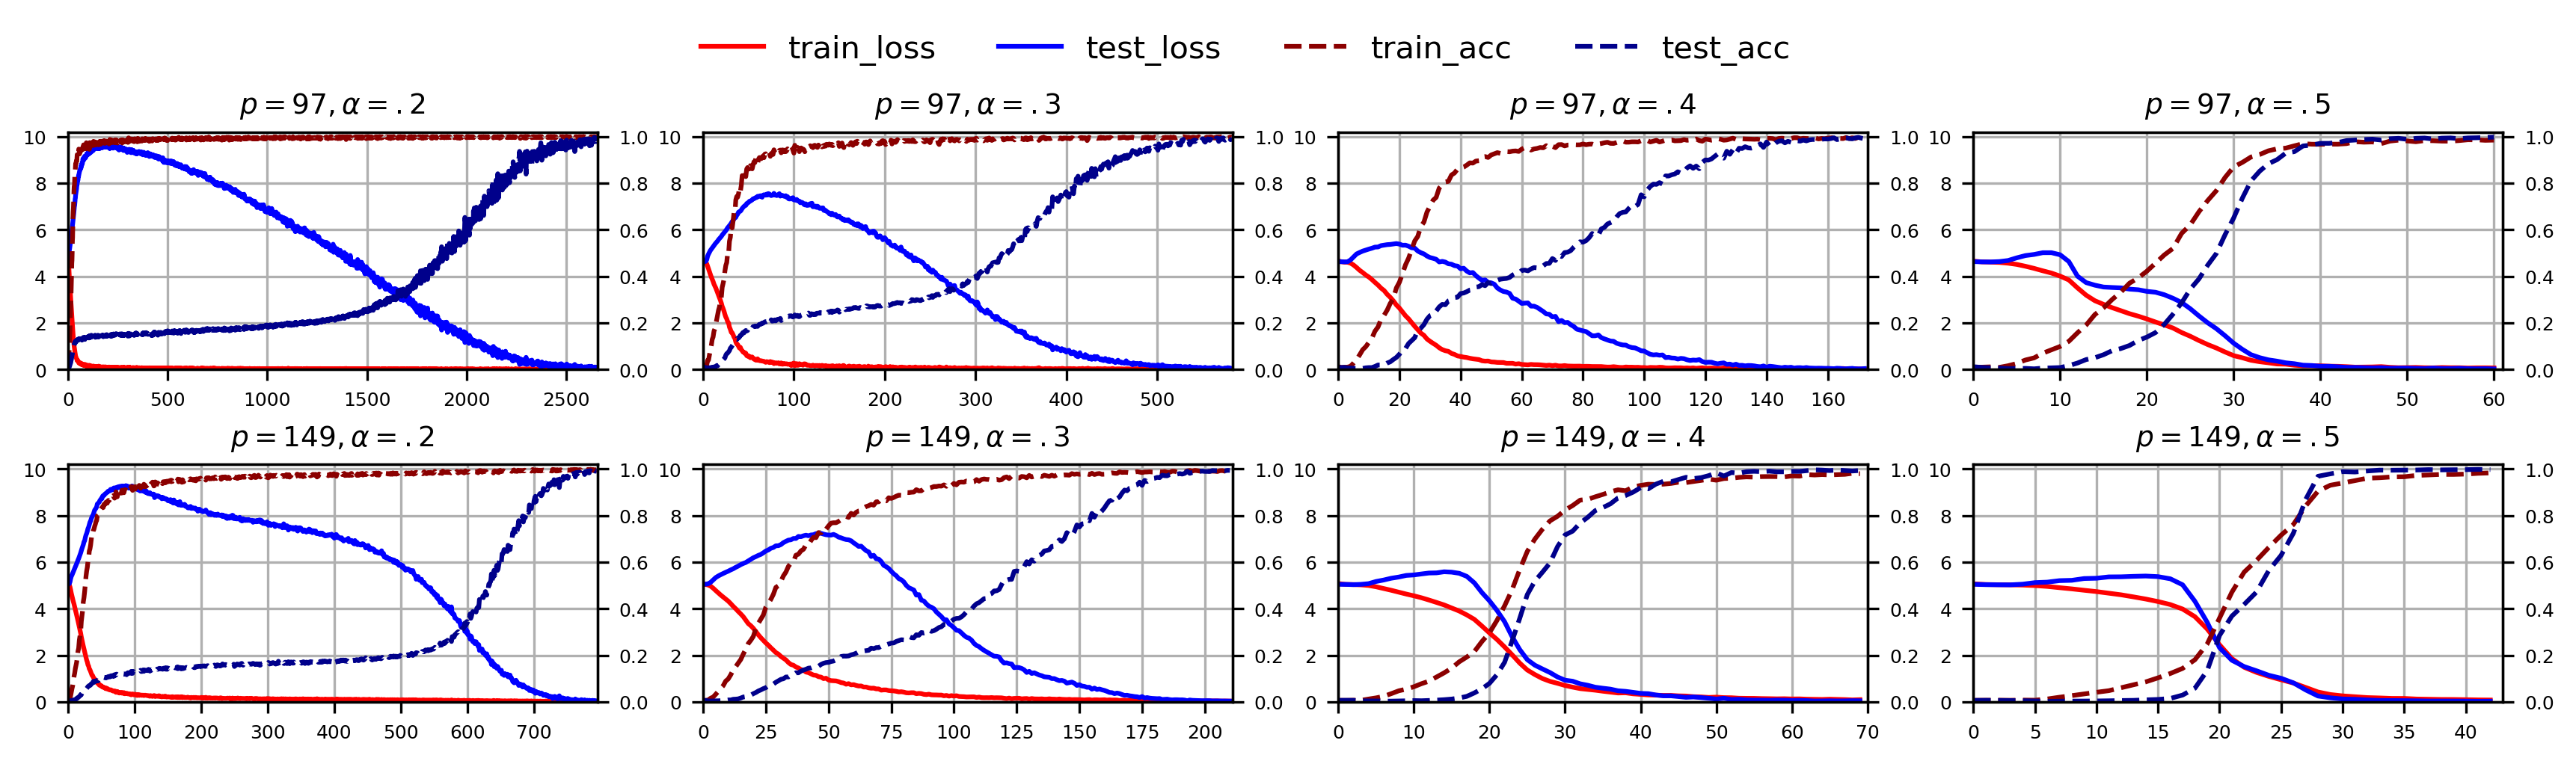
\includegraphics[width=\textwidth]{./pic/TSFM.png}
  \caption{Grokking on Transformers}
  \label{Grokking Transformers}
\end{figure}

\subsection{Grokking on MLP and LSTM}
\label{MLP}
We test the grokking phenomenon on the MLP and LSTM for $p = 97, 149$ and $\alpha = 0.3, 0.4, 0.5, 0.6$. $\eta$ is set $10^{-3}$ in most cases and is set a bit smaller in several tests to get convergent results. In detail, $\eta$ for (MLP, $p=97$, $\alpha=0.3$) is $7\times10^{-4}$ and for (MLP, $p=149$, $\alpha=0.6$) is $9\times10^{-4}$. The results are shown in Fig \ref{Grokking MLP} and \ref{Grokking LSTM}. We can see all models grok in learning with some difference as follows:

\begin{figure}[htbp]
  \centering
  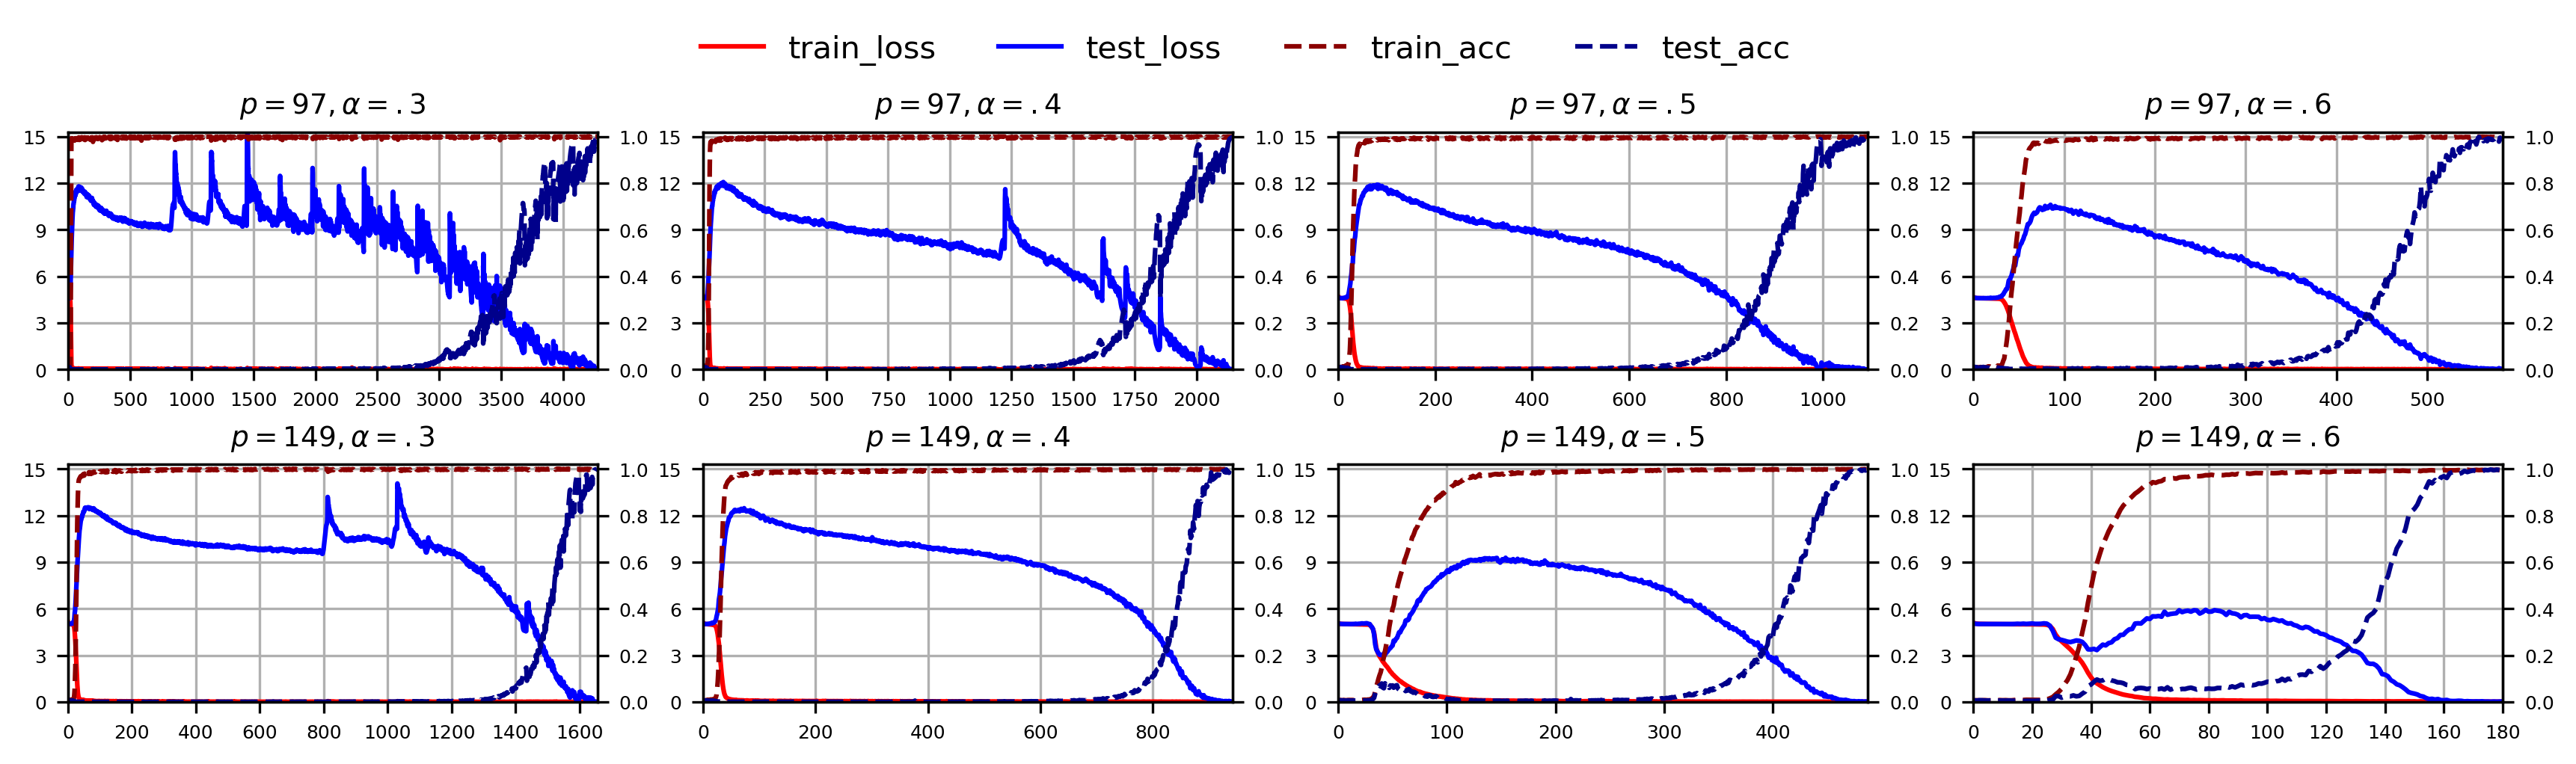
\includegraphics[width=\textwidth]{./pic/MLP.png}
  \caption{Grokking on MLP}
  \label{Grokking MLP}

  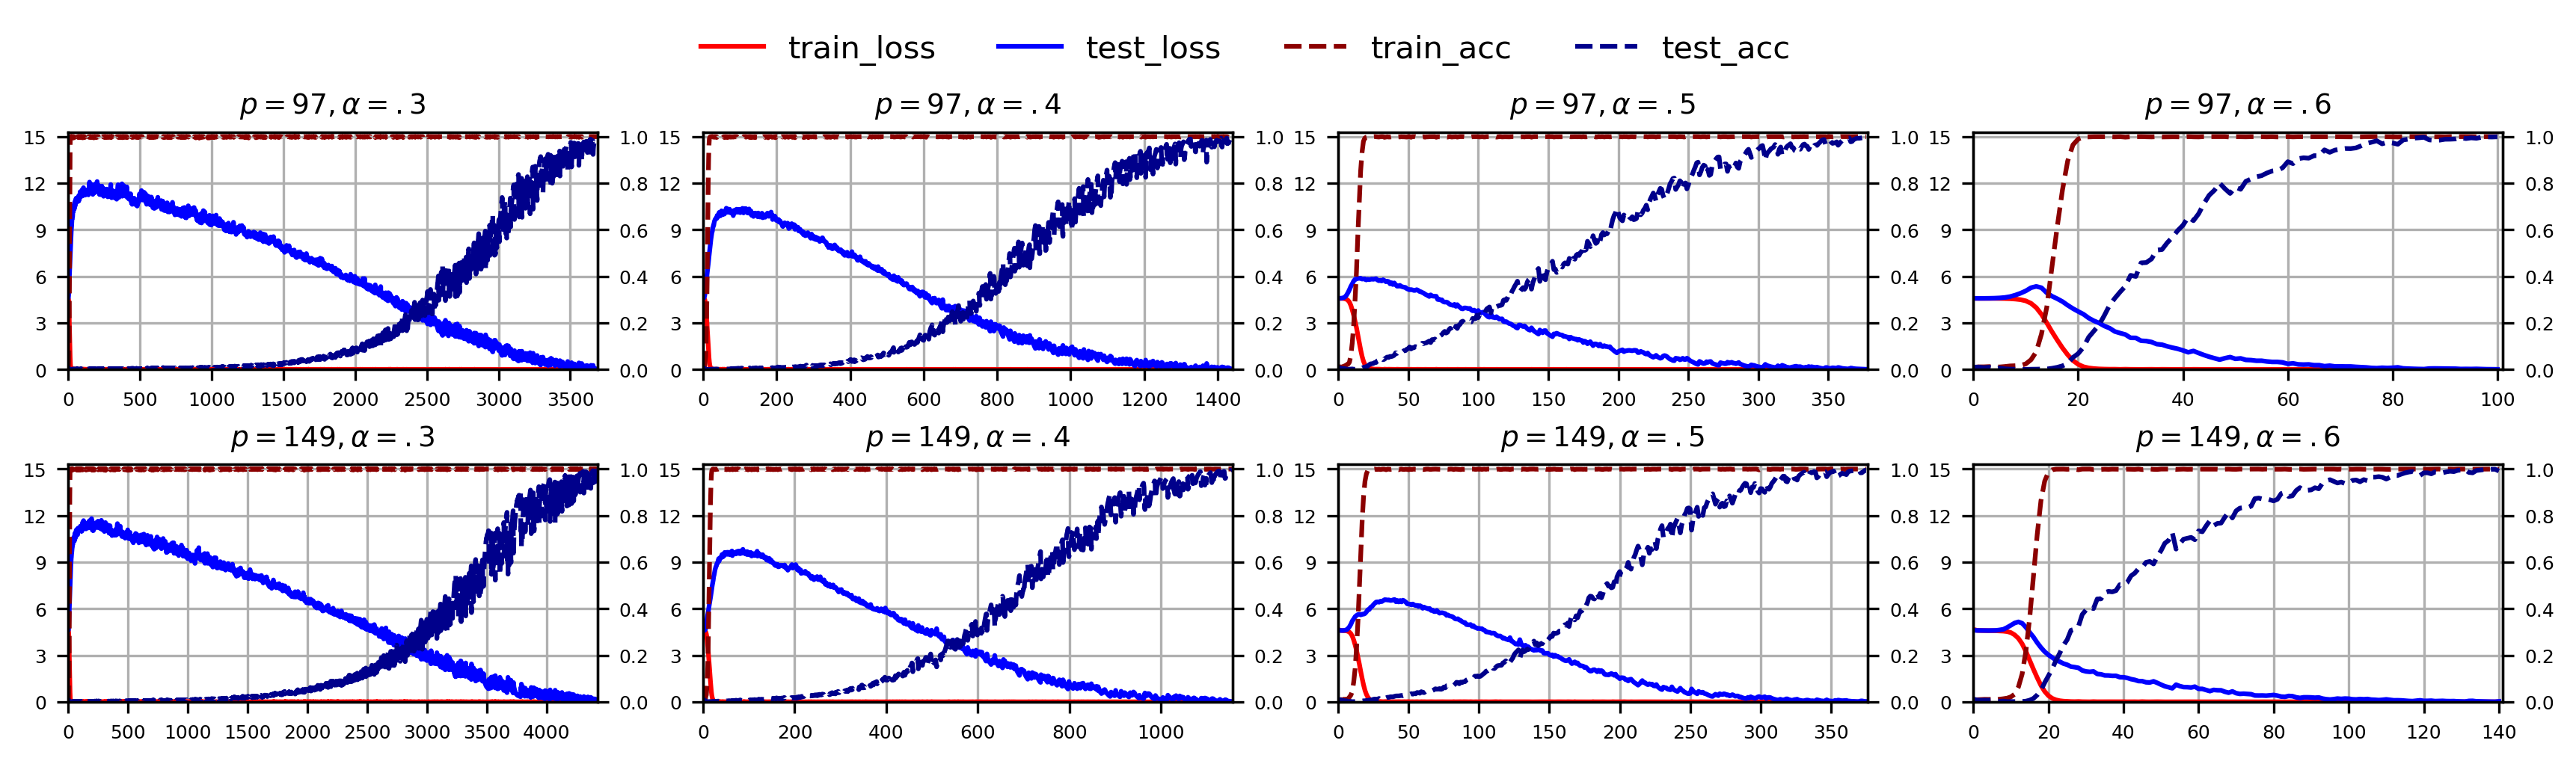
\includegraphics[width=\textwidth]{./pic/LSTM.png}
  \caption{Grokking on LSTM}
  \label{Grokking LSTM}
\end{figure}

\begin{itemize}
    \item Our Transformer and LSTM grok relatively slowly. After grokking, they need many epochs to reach 99\% accuracy. But for MLP, it needs much less epochs for the testing accuracy to increase to 99\% after grokking. This might be because the tokens are processed sequentially in Transformer and LSTM, while MLP processes them simultaneously.

    \item Before grokking, the testing accuracy of MLP and LSTM maintains at chance level. In contrast, the accuracy of Transformer remains at a relatively higher level (more than $10\%$) before it groks. The reason of this phenomenon will be explained in Subsection \ref{abel}.

    \item In all cases, we see that models with larger $p$ and $\alpha$ grok earlier. This is explicable, because the scale of $\mathcal{T}$ is about $\alpha p^2$. The larger $p$ or $\alpha$ is, the more data can be used for training. Hence, the model will converge more quickly.
\end{itemize}

\section{Impact of Different Optimizers and Regularization Methods}

In this section, we investigate the impact of different optimizers and regularization methods on the grokking phenomenon. We take Transformer as our model with $p = 97$ and $\alpha = 0.3$. For comparative purposes, the parameters are set with a batch size of $60$, a drop out of $0.1$ and a learning rate of $10^{-3}$. And we use AdamW as our benchmark optimizer, with $\beta_1 = 0.9,\ \beta_2 = 0.98$ and 0.05 weight decay. The results are shown in Fig \ref{optimizer}. We can preliminarily draw the following conclusion:

\begin{figure}[htbp]
  \centering
  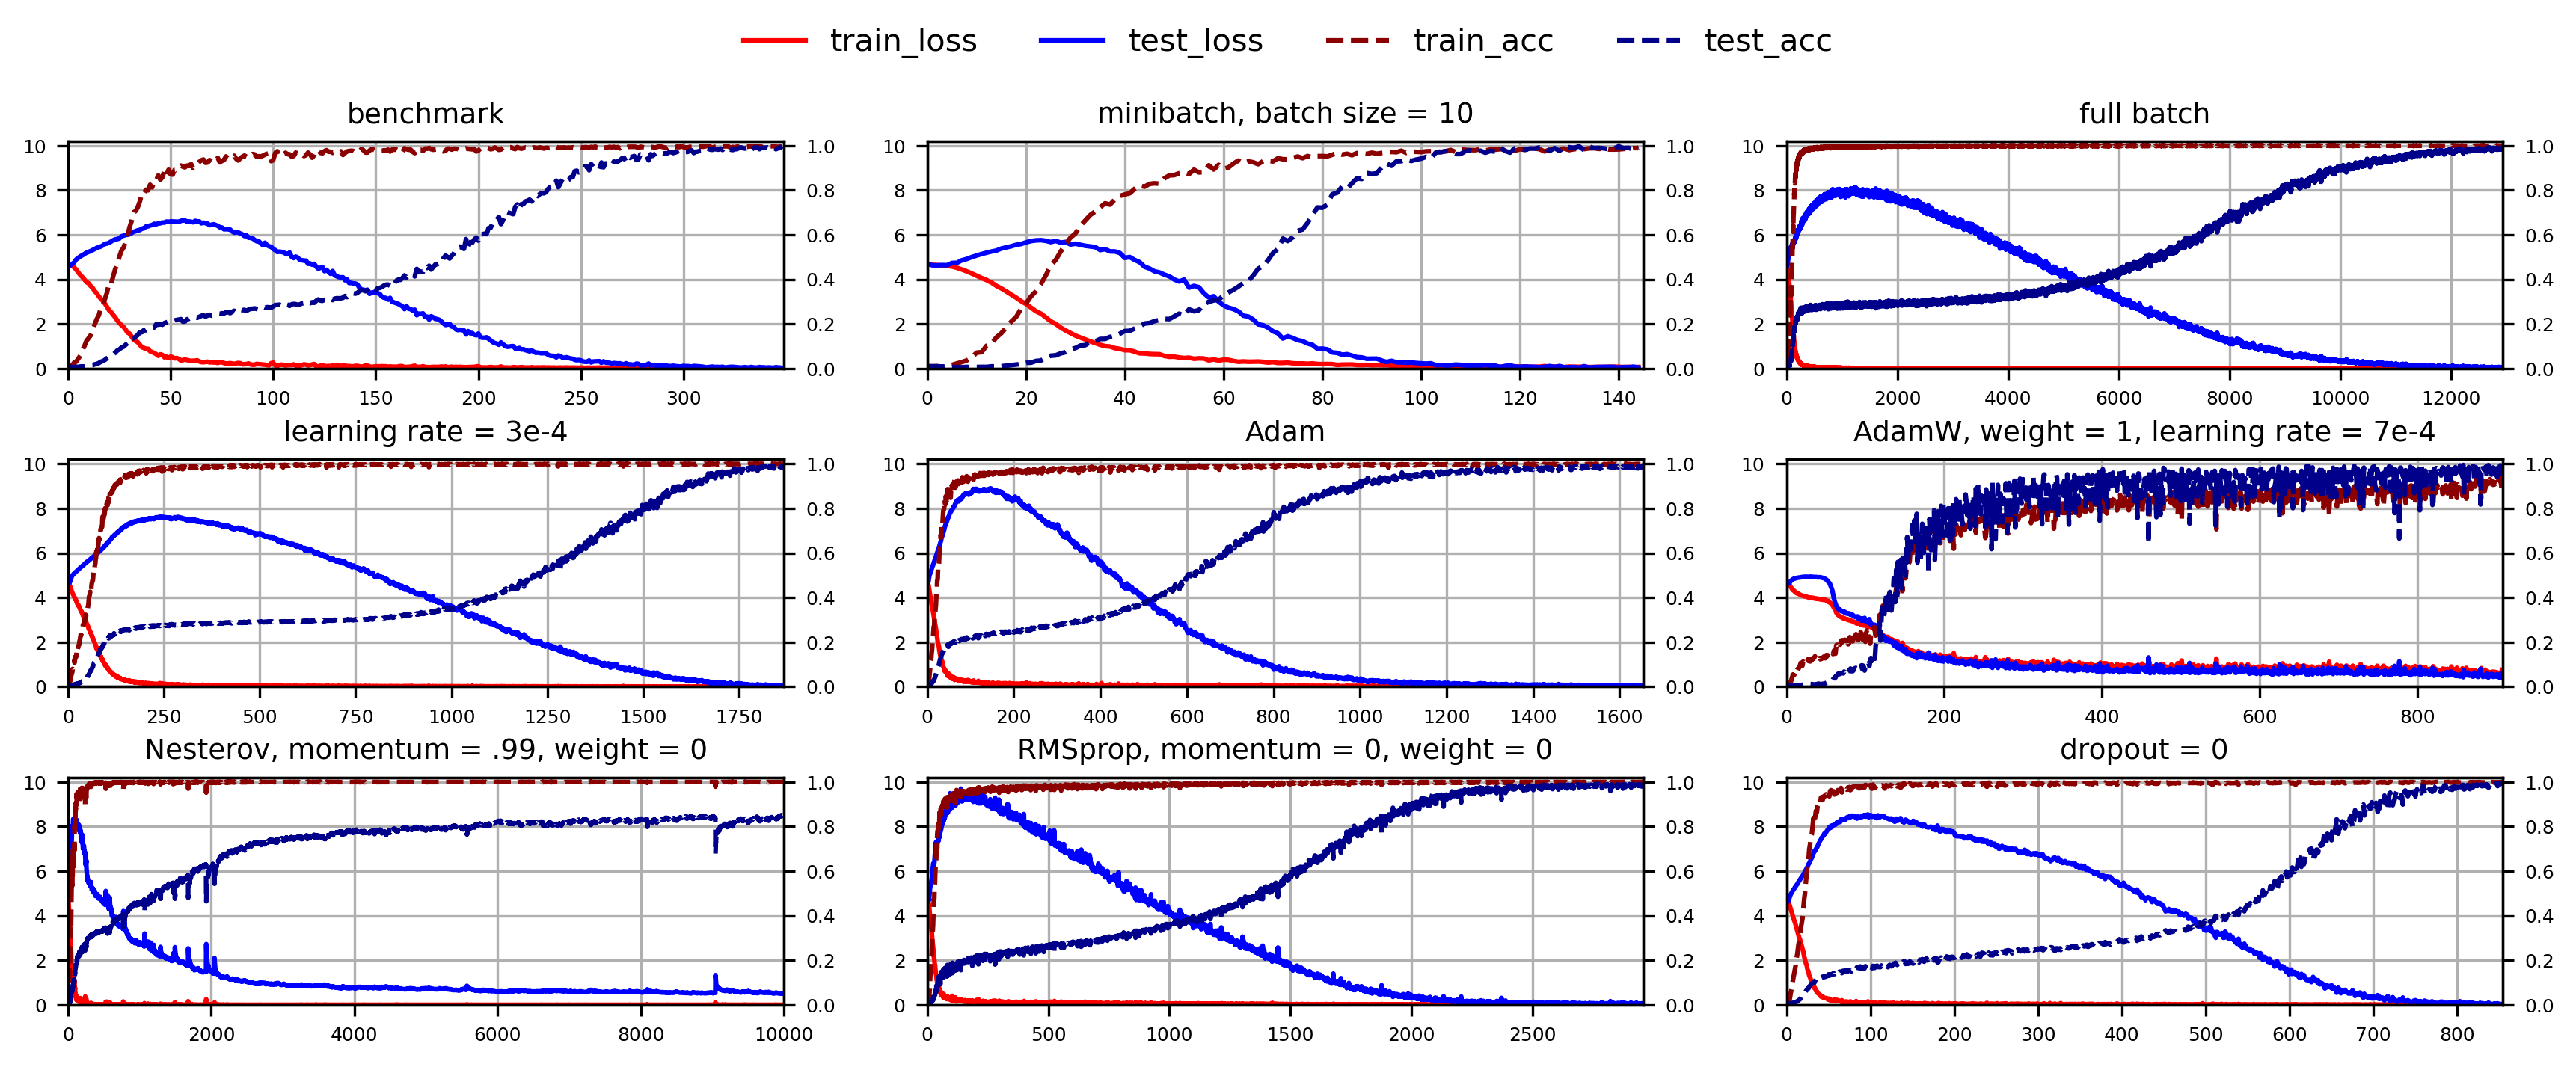
\includegraphics[width=\textwidth]{./pic/optimizer.png}
  \caption{Different Optimizers and Regularization Methods}
  \label{optimizer}
  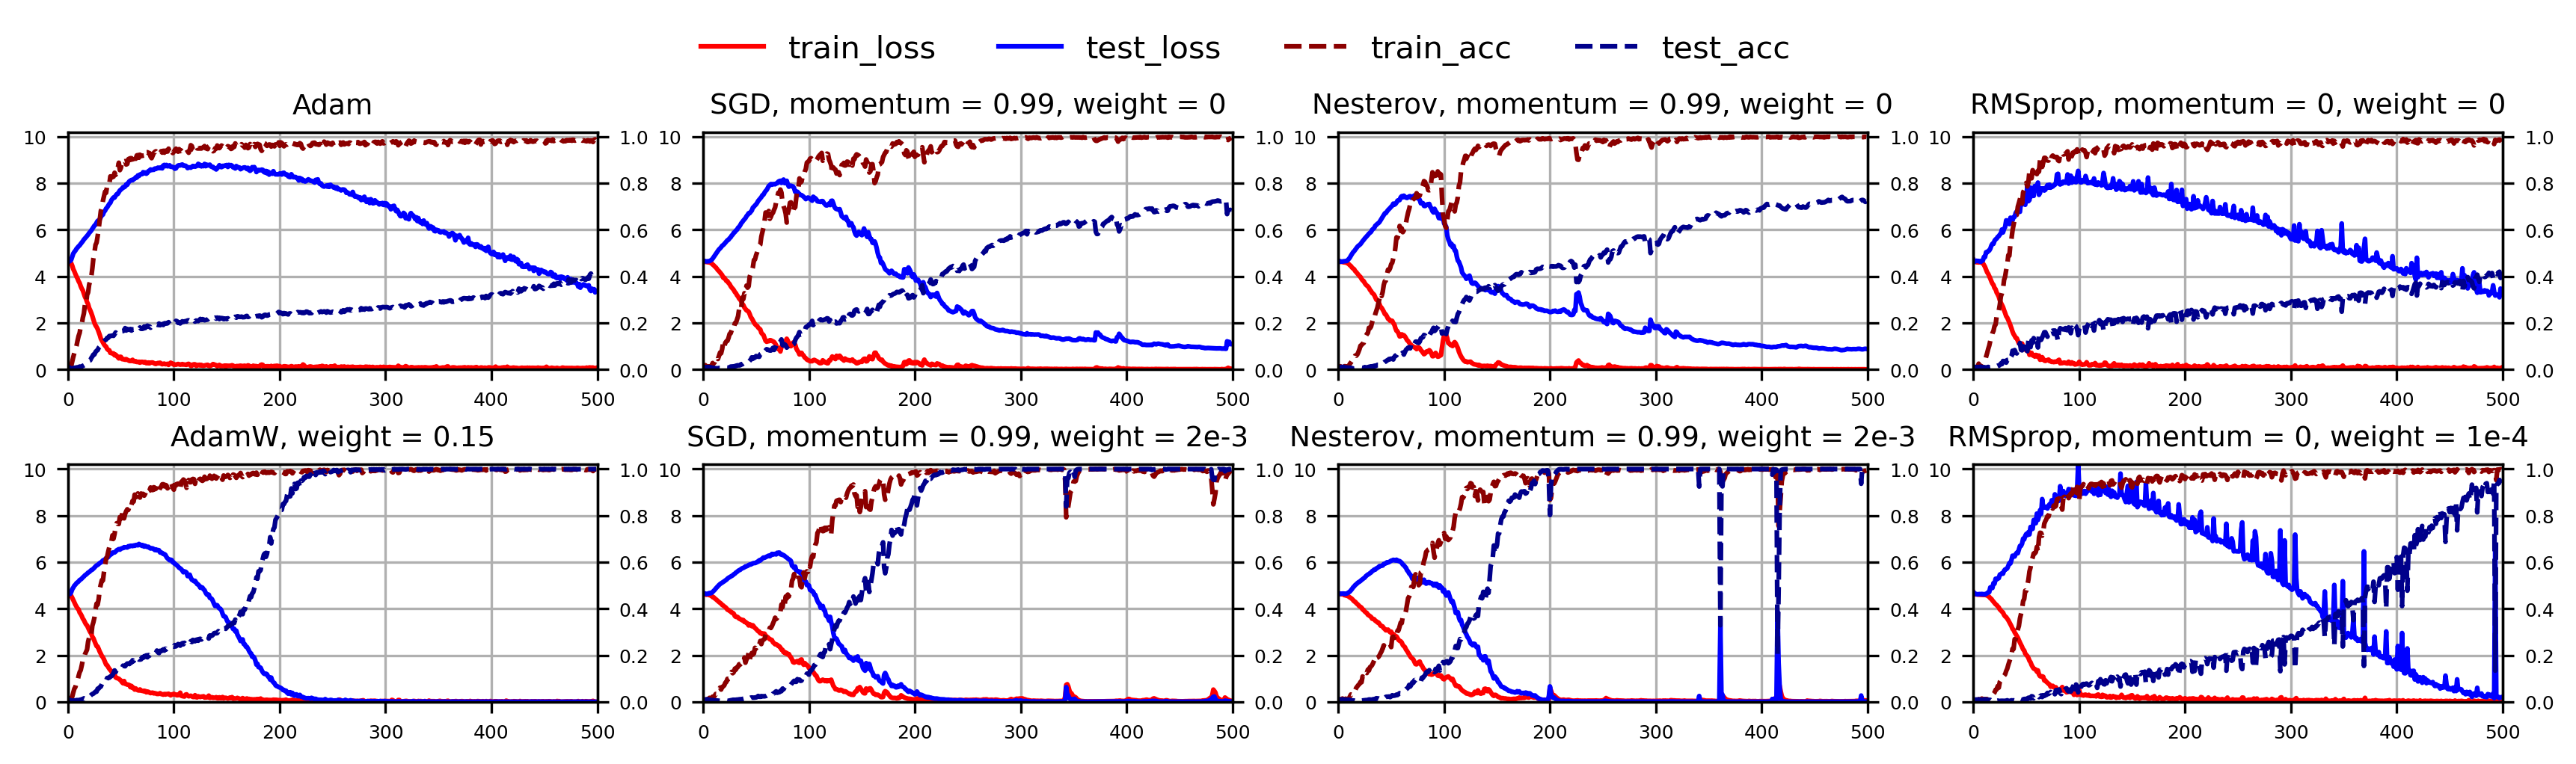
\includegraphics[width=\textwidth]{./pic/weight.png}
  \caption{Optimizers without and with Weights}
  \label{weight}
\end{figure}

\begin{itemize}
    \item A smaller batch size leads to faster convergence. This is easy to understand because the steps in an epoch are inversely proportional to the batch size.

    \item If no drop out is added in the model, it will converge much more slowly. Too small learning rate will cause the same problem.

    \item We test the grokking phenomenon on AdamW, SGD with Nesterov momentum and RMSprop. These optimizers always achieve convergence in their results over time.
    
    \item Moreover, we test the AdamW with different weights, including $0$ (AdamW with $0$ weight is exactly Adam), $0.05$ (benchmark model) and $1$ (here the learning rate is set a bit smaller to get faster convergence). The results imply that larger weights help to resolve the grokking. We did a further research into the influence of weights on different optimizers, including Adam, SGD momentum, Nesterov momentum and RMSprop. The total number of epochs is fixed at 500 and the results are plotted in Fig \ref{weight}. It is obvious that non zero weight decay will bring all optimizers better performance and faster grokking. Although larger weights might induce instability in the training process, it is still an effective method to relieve grokking. 
\end{itemize}

\section{Modular K-Summation}

\subsection{Datasets}

In this section we discuss the grokking phenomenon in modular $k$-summation: $\left(\overline{x_1}, \overline{x_2},\dots, \overline{x_k}\right) \mapsto \sum_{i=1}^k\overline{x_i}$ for $\overline{x_i} \in \mathbb{Z}_p$. So first we formalize the datasets for training and testing. It is worth noting that $+$ is not necessary in Sec \ref{Settings}. So based on the formalization in the case $k=2$, the dataset takes the form $\mathcal{D}_k = \lbrace \left(x_1, x_2,\dots, x_k, =\right)\left.\right| 0 \leqslant x_i \leqslant p-1\rbrace$, where the token of $=$ is still $p+1$ as before.

\subsection{Experiments}

We test the modular $k$-summation for $(k = 3, p = 47),\ (k = 4, p = 23),\ (k = 5, p = 11)$. Note that in these cases, the sizes of the datasets are 103,823, 279,841, 161,051, which are of about the same scale. We still use Transformer for training with the same parameters as in Sec \ref{models} with a batch size of 512. The results are displayed in Fig \ref{ksum}. We can see the grokking phenomenon still exists for $k$-summation, but it arises only when $\alpha$ is sufficient small. In fact, this verifies the hypothesis we proposed in Subsec \ref{MLP} that the grokking phenomenon is related to the scale of $\mathcal{T}$. The size of dataset in this section is about $10$ times larger than in Sec \ref{models}, hence the $\alpha$ is set about $10$ times smaller here. 

\begin{figure}[htbp]
  \centering
  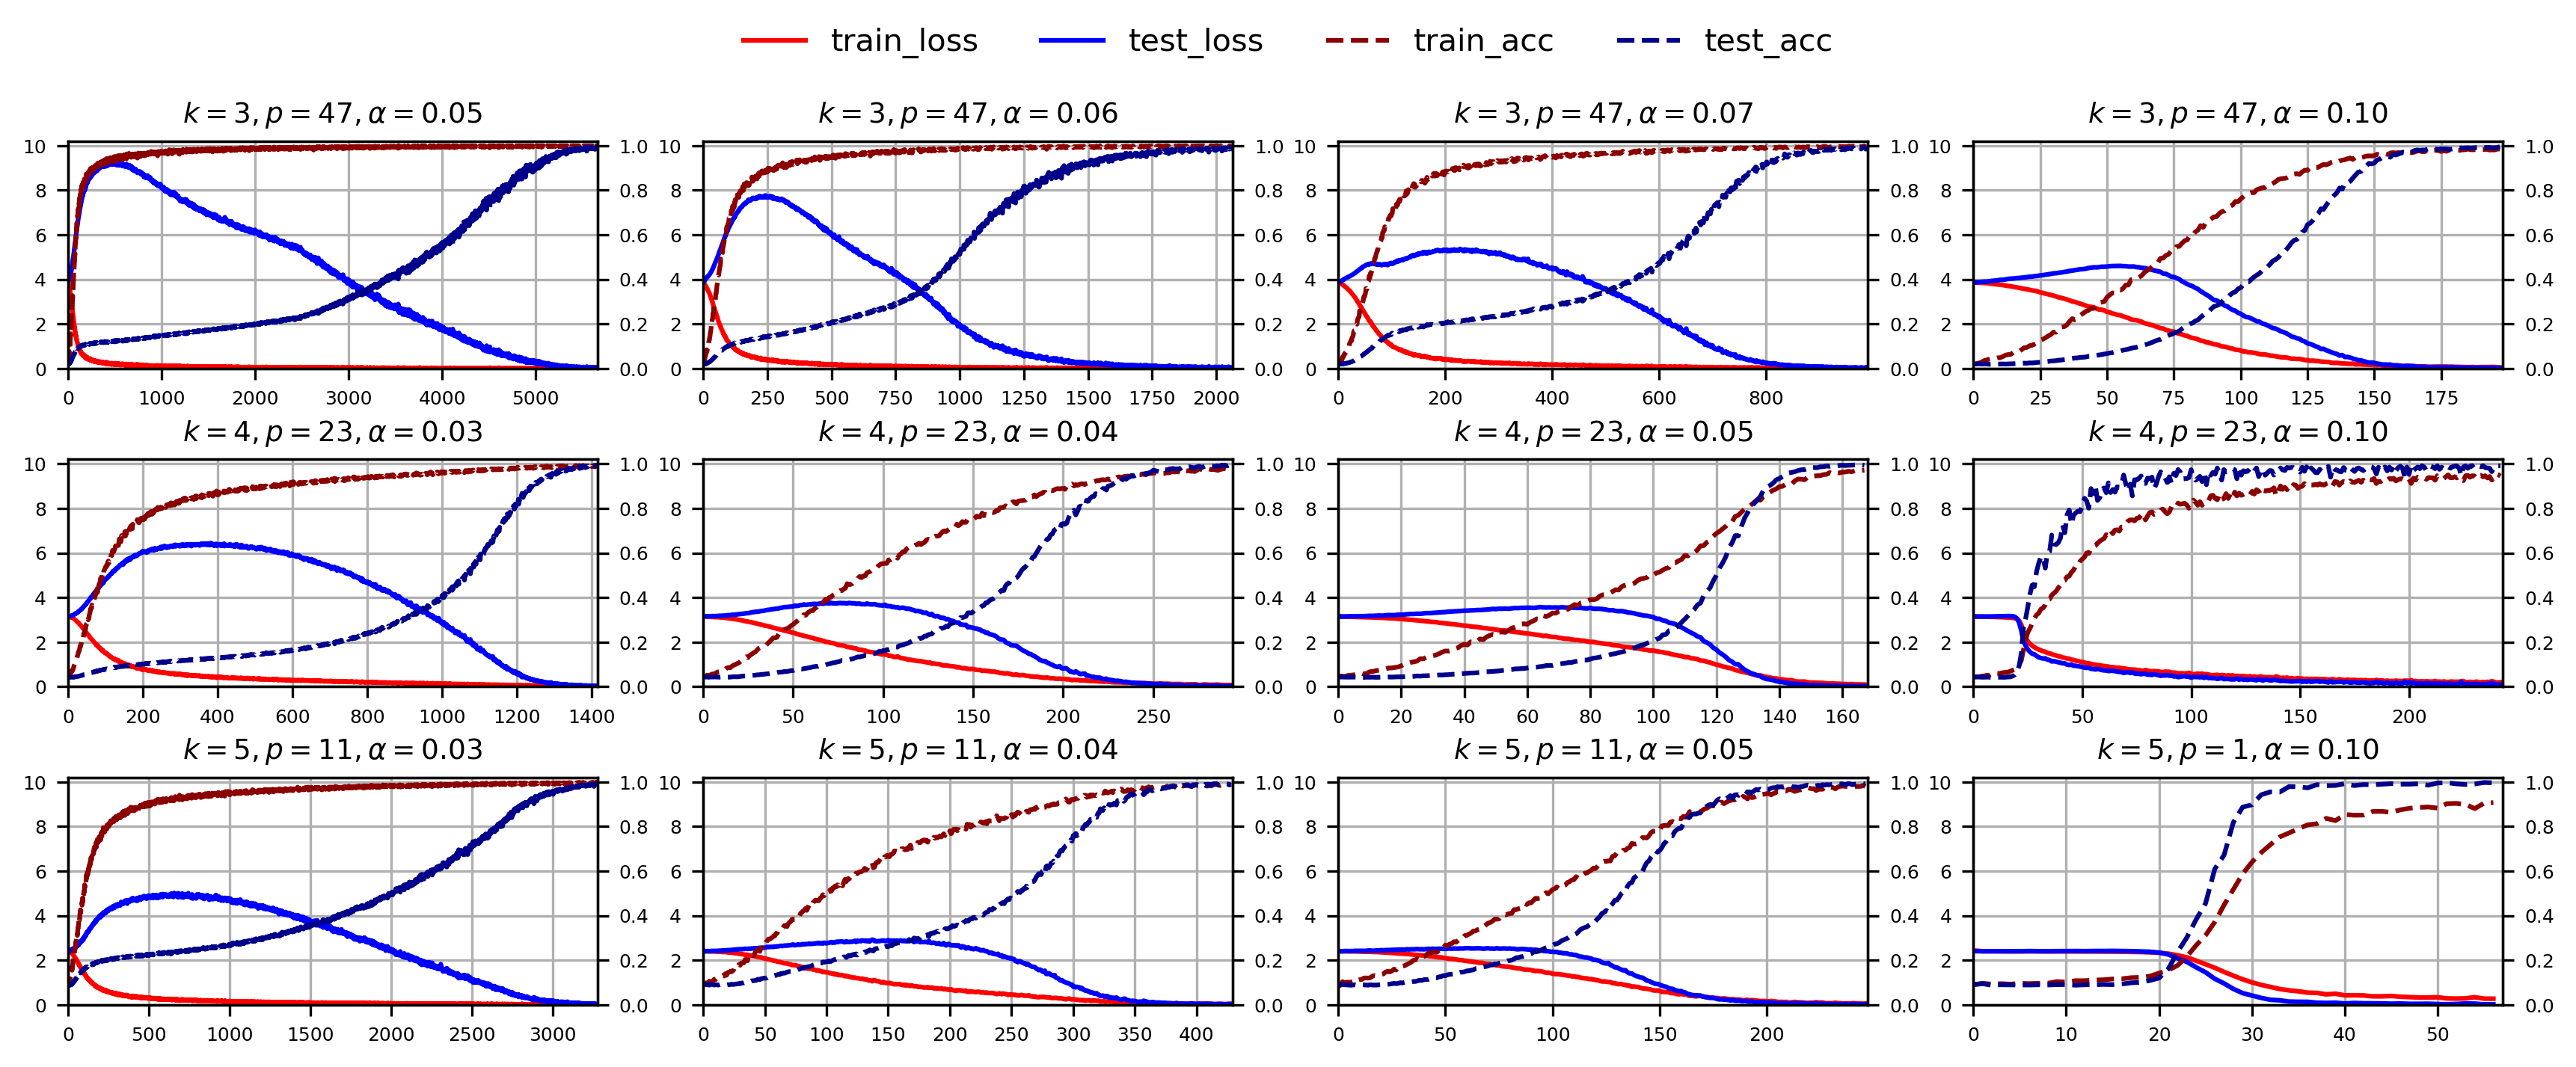
\includegraphics[width=\textwidth]{./pic/ksum.png}
  \caption{Modular K-Summation}
  \label{ksum}
\end{figure}

\section{Explanation of Grokking}

\subsection{Learning Process of the Properties of the Abelian Group}
\label{abel}

Since $(\mathbb{Z}_p, +)$ is an Abelian group, in this subsection we investigate into the learning process of several properties, including commutativity, associativity and the identity element. For commutativity, we test the accuracy of $\overline{x} + \overline{y} = \overline{y} + \overline{x}$ for all $\overline{x},\overline{y}\in\mathbb{Z}_p$. For identity element, we test the accuracy of $\overline{x} + \overline{0} = \overline{x}$ for all $\overline{x}\in\mathbb{Z}_p$. And for associativity, since it is too expensive to test all triples in $\mathbb{Z}_p^3$, we only randomly choose $N_{\text{assoc}}$ triples to test whether the identity $(\overline{x} + \overline{y}) + \overline{z} = \overline{x} + (\overline{y} + \overline{z})$ holds.

We explore the learning process in Transformer and MLP. For the training set $\mathcal{T}$, we define its "complement" as $\mathcal{C_T} = \lbrace \left.(\overline{x}, \overline{y})\ \right|\ (\overline{x}, \overline{y}) \notin \mathcal{T}\ \text{and}\ (\overline{y}, \overline{x}) \in \mathcal{T}\rbrace$. Obviously $\mathcal{C_T} \subset \mathcal{V}$. We test the accuracy on $\mathcal{C_T}$ and $\mathcal{V}\backslash\mathcal{C_T}$ to examine the learning of commutativity. We first test the case $\mathcal{C_T} = \varnothing$, which means $\mathcal{T}$ is symmetric with respect to $\overline{x}$ and $\overline{y}$. Meanwhile, we design a test to eliminate all tuples containing $\overline{0}$ from $\mathcal{T}$ while maintaining $\alpha$ unchanged. That is, $\mathcal{Z}_0(\mathcal{T}\cup\mathcal{C_T}) = \varnothing$ where $\mathcal{Z}_q(\mathcal{S}) = \lbrace(\overline{x},\overline{q}) \in \mathcal{S}\rbrace$. Our purpose is to see how the structure of $\mathcal{T}$ effects the learning. We use $(\text{Transformer}, p = 97, \alpha = 0.25)$ and $(\text{MLP}, p = 97, \alpha = 0.5)$ with the same parameters as in Sec \ref{models}. $N_\text{assoc}$ is set $10\ 000$ and results are shown in Fig \ref{adding}. We observe some interesting phenomena here.

\begin{figure}[htbp]
  \centering
  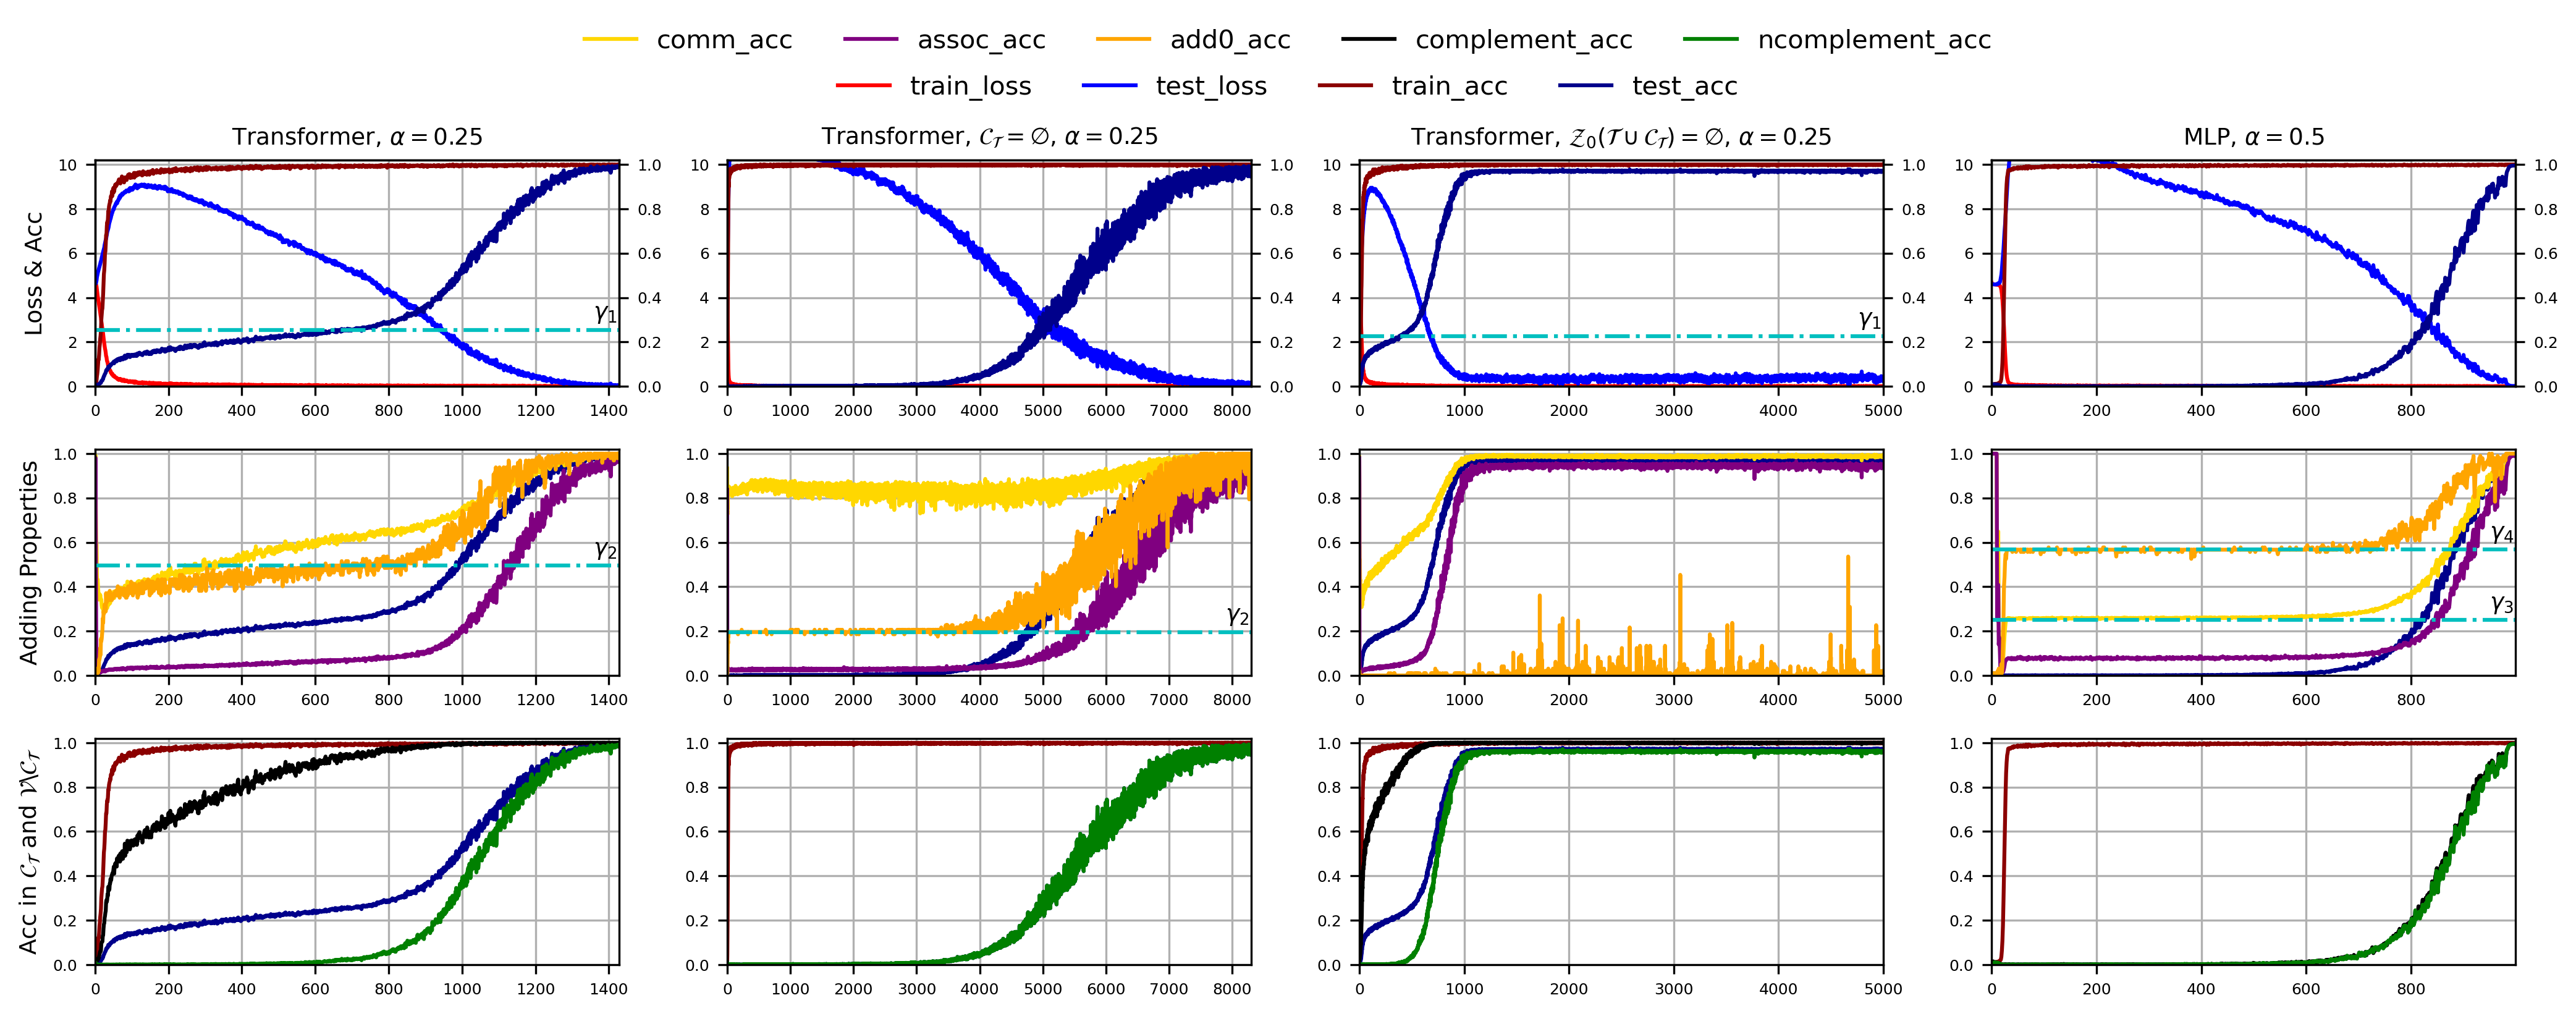
\includegraphics[width=\textwidth]{./pic/add.png}
  \caption{Learning of Adding Properties. \textbf{Top.} Loss and accuracy. $\gamma_1 = \#\mathcal{C_T} /\#\mathcal{V}$. \textbf{Mid.} Accuracy of the three properties: commutativity, associativity and the identity element. $\gamma_2 = \#\mathcal{Z}_0(\mathcal{T}\cup\mathcal{C_T}) / \#\mathcal{Z}_0(\mathcal{D}),\ \gamma_3 = \#\mathcal{A_T}/\#\mathcal{D},\ \gamma_4 = \#\mathcal{Z}_0(\mathcal{T})/\#\mathcal{Z}_0(\mathcal{D})$. \textbf{Bottom.} Accuracy on $\mathcal{T}, \mathcal{V}, \mathcal{C_T}, \mathcal{V}\backslash\mathcal{C_T}$}
  \label{adding}
\end{figure}

\begin{itemize}
    \item \textbf{Transformer learns the modular addition is Abelian before knowing what the modular addition is}. This sounds like a classic French joke, but it just works. From row 1 in Fig \ref{adding} we see the accuracy on $\mathcal{C_T}$ improves much more quickly that on $\mathcal{V}\backslash\mathcal{C_T}$. Recall that in Sec \ref{models} we see the testing accuracy of Transformer maintains at a relatively high level before it groks. Now we that this accuracy comes from the $\mathcal{C_T}$ part, and the level is exactly $\#\mathcal{C_T} /\#\mathcal{V}$.

    This helps to give an explanation of the grokking phenomenon on Transformer. At first, the model learns to fit $\mathcal{T}$ and generalizes to $\mathcal{C_T}$ quickly. In this stage, the testing accuracy gradually improves to $\gamma_1 = \#\mathcal{C_T} /\#\mathcal{V}$. When the accuracy on $\mathcal{C_T}$ is sufficient high, the model begins to generalize to $\mathcal{V}\backslash\mathcal{C_T}$. That is when the model groks. The whole learning process can be divided into three parts as follows:
    \begin{align}
        \mathcal{T} \rightarrow \mathcal{C_T} \xrightarrow{\text{Grok!}} \mathcal{V}\backslash\mathcal{C_T}\label{3step}
    \end{align}
    In fact, this phenomenon in row 1 of Fig \ref{adding} is not accidental, and two learning steps \eqref{3step} widely exists in experiments. We repeat several experiments in \ref{appendix-repeat} to demonstrate this.

    \item \textbf{The learning process depends on $\mathcal{T}$}. We first have a look at the case $\mathcal{C_T} = \varnothing$ (row 2 in Fig \ref{adding}). From the results we see the testing accuracy is zero before grokking. This is consistent with \eqref{3step}, since $\gamma_1 = \#\mathcal{C_T} /\#\mathcal{V} = 0$. Besides, it takes more epochs for the model to converge, because $\mathcal{T}$ is closed under symmetry and it is more difficult to generalize from $\mathcal{T}$ to $\mathcal{V}$. However, despite the low testing accuracy, the accuracy of commutativity is extremely high in the whole process. This means although the model does not know what $\overline{x}+\overline{y}$ is, it learns quickly that $\overline{x}+\overline{y} = \overline{y}+\overline{x}$.
    
    \begin{figure}[htbp]
      \centering
      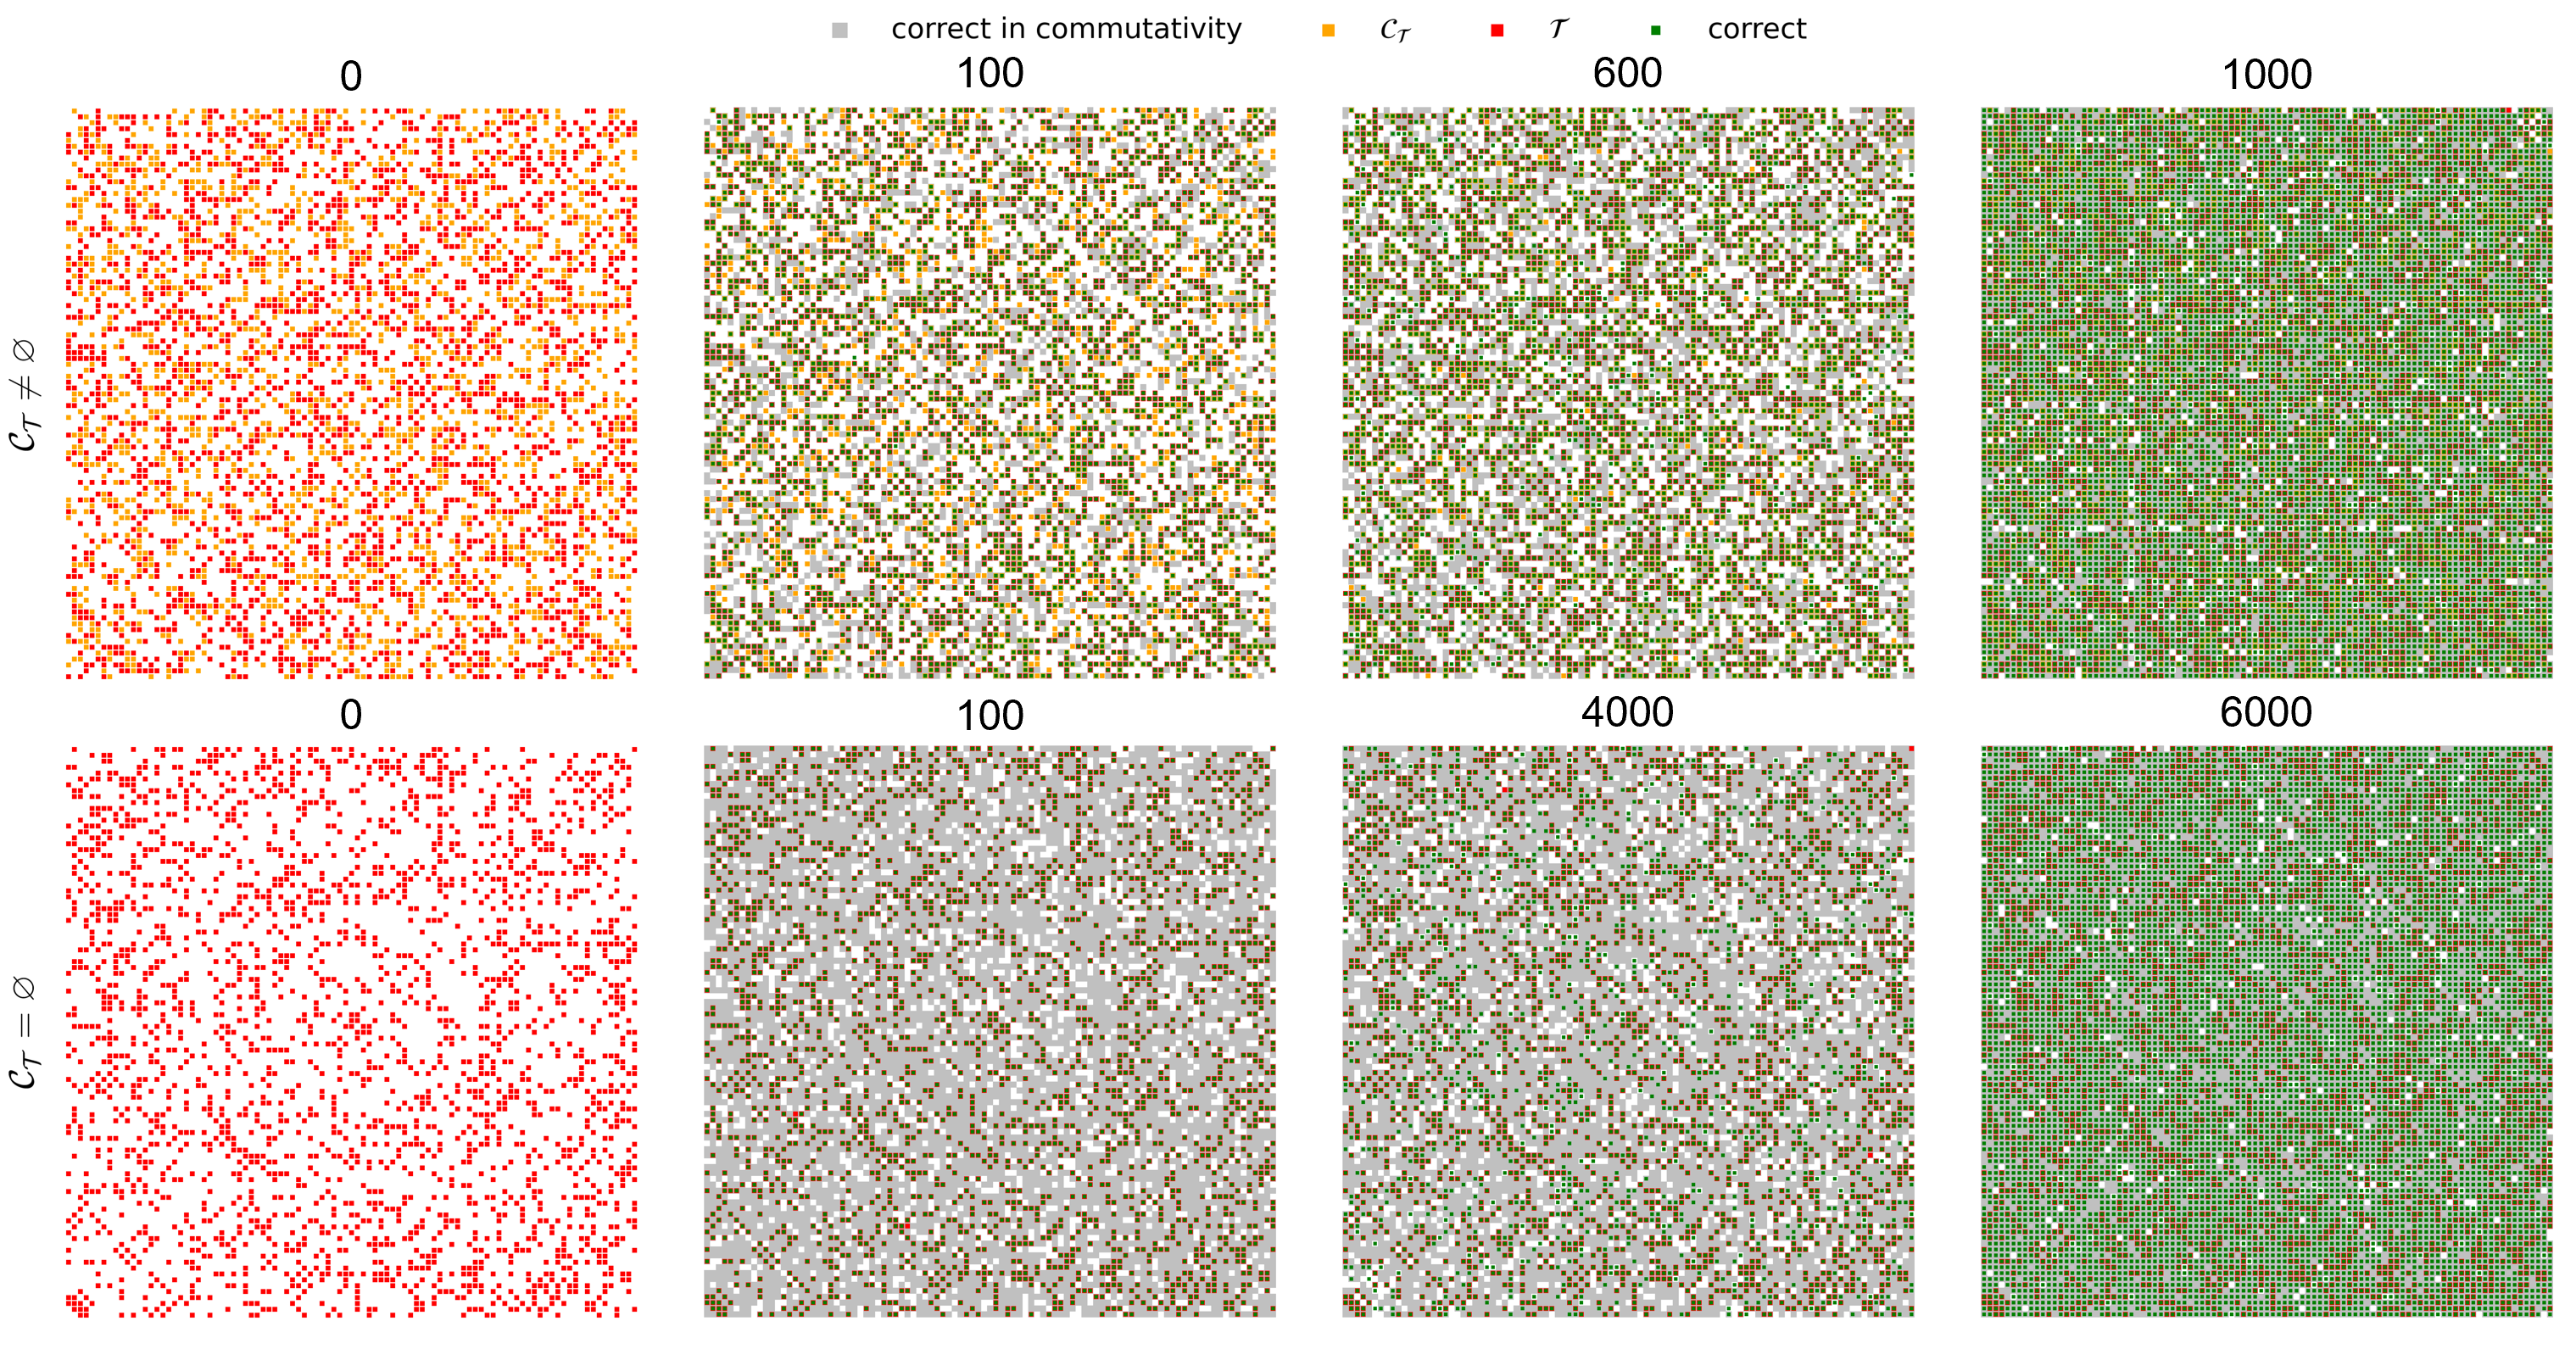
\includegraphics[width=\textwidth]{./pic/grid.png}
      \caption{Prediction on $\mathcal{D}$ when $\mathcal{C_T} \neq \varnothing$ and $\mathcal{C_T} = \varnothing$}
      \label{grid}
      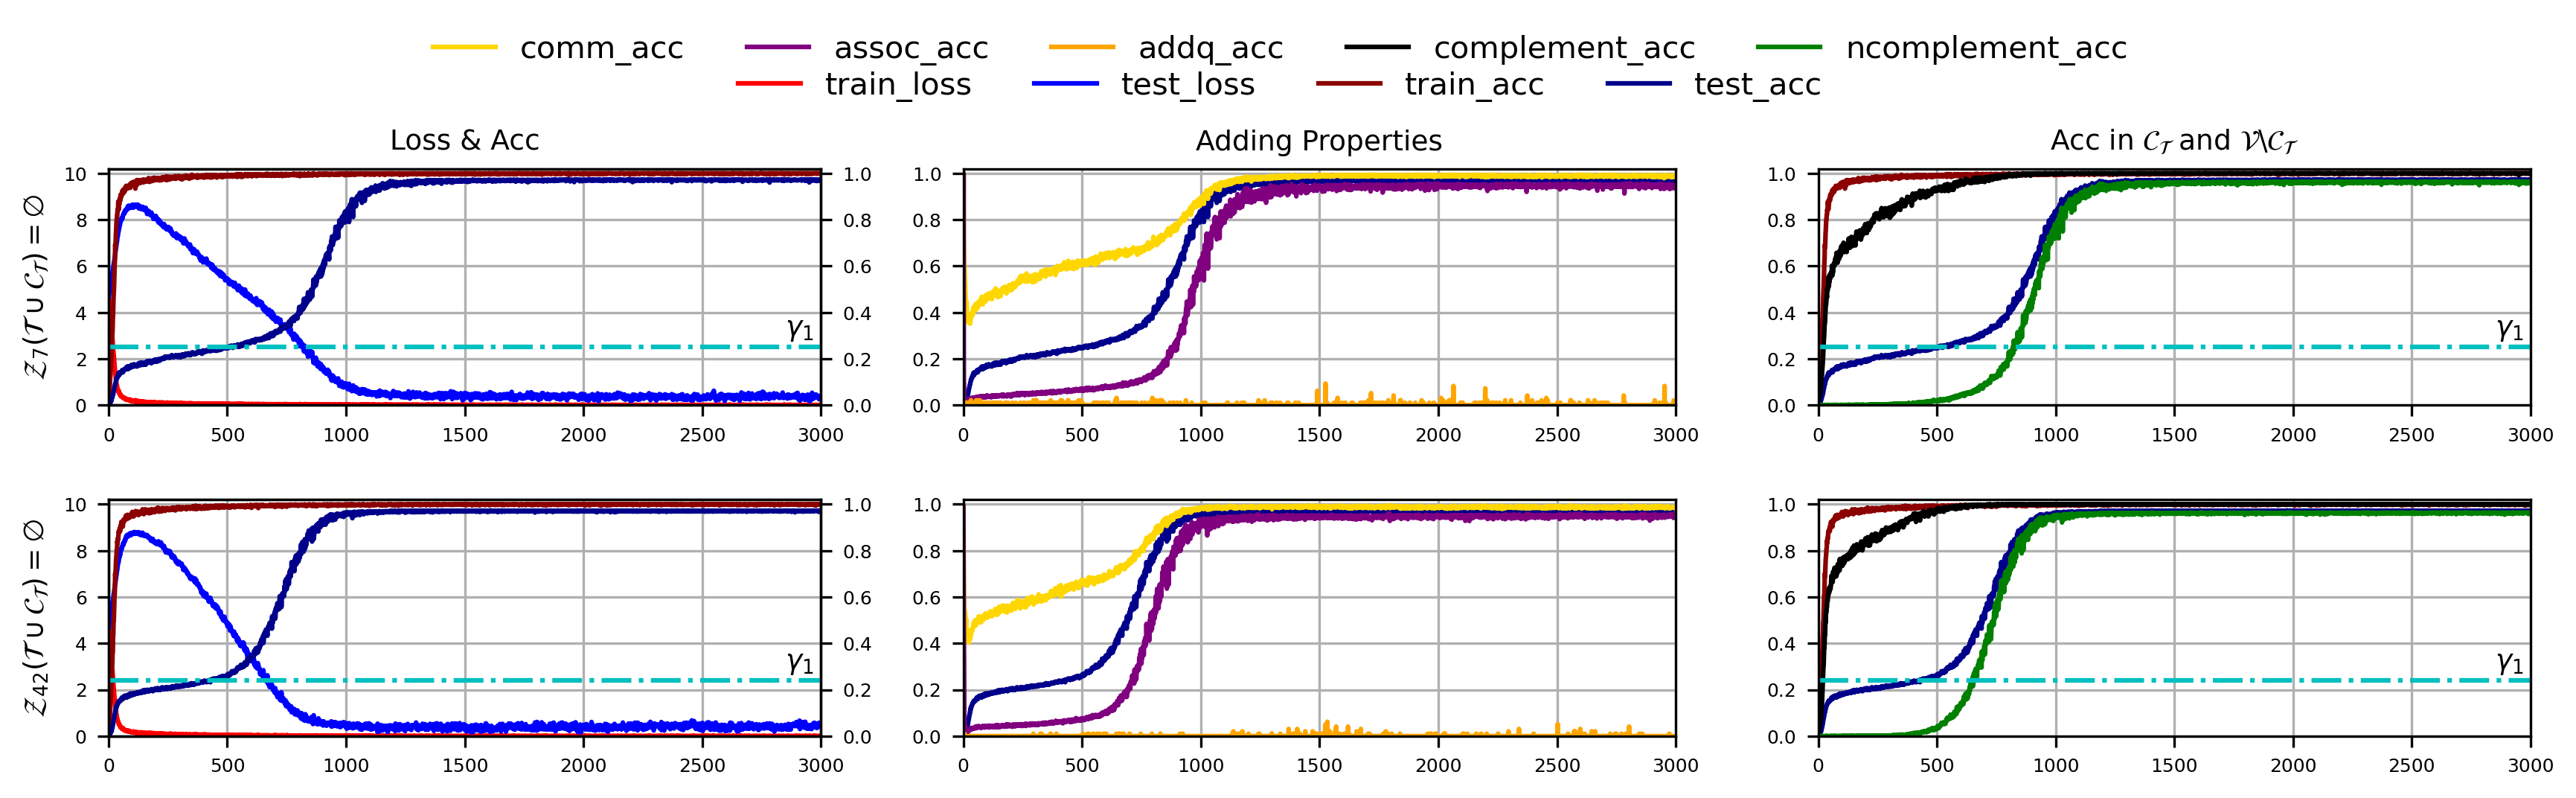
\includegraphics[width=\textwidth]{./pic/noq.png}
      \caption{$\mathcal{Z}_7(\mathcal{T}\cup\mathcal{C_T}) = \varnothing$ and $\mathcal{Z}_{42}(\mathcal{T}\cup\mathcal{C_T}) = \varnothing$}
      \label{noq}
    \end{figure}
    For a more precise observation, we focus on the model's prediction on each sample in $\mathcal{D}$. We use a colored $p\times p$ grid to represents $\mathbb{Z}_p^2$. The samples in $\mathcal{T}$ and $\mathcal{C_T}$ are represented by $\ColorSquare{251, 0, 6}{2mm}$ and $\ColorSquare{254, 148, 6}{2mm}$ separately. The correctly predicted samples are represented by $\ColorSquare{17, 112, 0}{1.5mm}$. We say a sample $(\overline{x}, \overline{y})$ is "correct in commutativity" if the model $\mathcal{M}$ predicts that $\mathcal{M}(\overline{x}, \overline{y}) = \mathcal{M}(\overline{y}, \overline{x})$, which is represented by $\ColorSquare{179, 179, 179}{2.5mm}$. We test $\mathcal{C_T} \neq \varnothing$ and $\mathcal{C_T} = \varnothing$ for $\alpha=0.25$ and plot the results in Fig \ref{grid}.

    For $\mathcal{C_T} \neq \varnothing$, the model fits $\mathcal{T}$ at about 100 epochs and generalizes to $\mathcal{C_T}$ at about 600 epochs (see \ref{appendix-grid} for details). This can be verified by Fig \ref{grid}. At 100 epochs, the model performs well only on $\mathcal{T}$. At 600 epochs, almost all samples in $\mathcal{C_T}$ are predicted correctly. This again confirms that the learning is progressive and step-by-step. And when $\mathcal{C_T} = \varnothing$, it only needs 100 epochs to obtain a high accuracy in commutativity, but the model generalizes to $\mathcal{V}$ only after thousands of epochs. To get faster convergence, $\mathcal{T}$ should not be very "symmetric".
    
    As of $\overline{0}$ addition, we can see that for general $\mathcal{T}$ (row 1, 2 in Fig \ref{adding}), the accuracy of $\overline{0}$ addition increases to $\gamma_2 = \#\mathcal{Z}_0(\mathcal{T}\cup\mathcal{C_T}) / \#\mathcal{Z}_0(\mathcal{D})$ in the first stage. This is consistent with \eqref{3step}. However, as we see in the case $\mathcal{Z}_0(\mathcal{T}\cup\mathcal{C_T}) = \varnothing$, the accuracy of $\overline{0}$ addition remains zero in the whole experiment. Since $\mathcal{Z}_0(\mathcal{T}\cup\mathcal{C_T}) = \varnothing$, it is reasonable the accuracy is zero at first. But it is interesting that the model never learns what $\overline{0}$ is or how to calculate $\overline{x} + \overline{0}$.  In fact, this is also true for $\overline{q}$ other than $\overline{0}$. We test the case $\mathcal{Z}_7(\mathcal{T}\cup\mathcal{C_T}) = \varnothing$ and $\mathcal{Z}_{42}(\mathcal{T}\cup\mathcal{C_T}) = \varnothing$ on $(\text{Transformer}, p = 97, \alpha = 0.25)$ as in Fig \ref{noq}. Again the model has no idea what $\overline{q}$ is and the accuracy of $\overline{q}$ addition maintains at chance level.
    
    To some extent, these experiments reveal that a proper $\mathcal{T}$ is necessary for the model to generalize fast and perform well. At least all elements in $\mathbb{Z}_p$ must appear once in $\mathcal{T}$.

    \item \textbf{MLP groks differently from Transformer}. In contrast to the Transformer, we can see that the accuracy of $\mathcal{C_T}$ and $\mathcal{V}\backslash\mathcal{C_T}$ changes simultaneously for MLP. If we let $\mathcal{A_T} = \lbrace\left.(\overline{x}, \overline{y})\ \right|\ (\overline{x}, \overline{y}) \in \mathcal{T}\ \text{and}\ (\overline{y}, \overline{x}) \in \mathcal{T}\rbrace$, we can see that the accuracy for commutativity keeps $\gamma_3 = \#\mathcal{A_T}/\#\mathcal{D}$ and the accuracy for $\overline{0}$ addition maintains at $\gamma_4 = \#\mathcal{Z}_0(\mathcal{T})/\#\mathcal{Z}_0(\mathcal{D})$, which means that MLP cannot generalize any of the properties to the testing dataset before grokking. This partly explains why the testing accuracy of MLP remains at chance level and verifies the advantages of Transformer over MLP.
\end{itemize}

\subsection{Frequencies of the Last Layer}

From the Fig 3 in \cite{power2022grokking}, we see that the t-SNE projection of output layer weights is regularly arranged in $\mathbb{R}^2$. We have a detailed exploration into this phenomenon. For all models in Sec \ref{Settings}, the output layer is linear with weights $\bm{W} \in \mathbb{R}^{p\times d}$. Each row of $\bm{W}$ can be viewed as a representation of $\overline{x}$ in latent space. We denote the representation for $\overline{i}$ as $\bm{w}_i$. By t-SNE, $\bm{w}_i$ is transformed into $\widehat{\bm{w}}_i \in \mathbb{R}^2$. Consider $\widehat\Delta_i = \widehat{\bm{w}}_i - \widehat{\bm{w}}_{i-1}$, \cite{power2022grokking} shows that approximately we have $\widehat\Delta_i = re^{\frac{2ik\pi}{p}}$ for some $k$ and $r$. Hence, we consider to do DCT on the $x$ component of $\widehat\Delta_i$ and monitor how the frequencies change in the training process. It is hoped that all frequencies approach zero except two ($\frac{2k\pi}{p}, \frac{2(p-k)\pi}{p}$). In fact, we have $\widehat\lambda_s = \widehat\lambda_{p-s}$ (see \ref{appendix-notation}) and we only need to focus on the low frequencies for $s \leqslant \lceil\frac{p}2\rceil$.

Besides, we try to investigate the "frequency" change of $\bm{w}_i$ directly. It is not that convenient to do DCT in $\mathbb{R}^p$ , so we turn to do DCT on the inner production between $\bm{w}_i$s. In detail, let $\Delta_i = \bm{w}_i - \bm{w}_{i-1}$, $a_{ij} = \langle\Delta_i, \Delta_j\rangle_2$ be the inner production and $l_k = \sum_{\overline{j}-\overline{i}=\overline{k}}a_{ij} /p$ be the average. $l_k$ is induced because the matrix $A = (a_{ij})$ is becoming "circulant" finally (see \ref{appendix-circulant}). Again, we do DCT on $l_i$s to get the frequencies $\lambda_i$, and we still only need to focus on the low frequencies.

We use two gauges to measure the similarity between $\bm\lambda\ (\text{or}\ \bm{\widehat\lambda})$ and the unit vector $\bm e_i$: Signal Noise Ratio (SNR) and Entropy. They take the form
\begin{align}
    \text{SNR}(\bm\lambda) = \frac{\lVert \bm\lambda\rVert_1}{\lVert \bm\lambda\rVert_2},\ \text{Entropy}(\bm\lambda) = -\sum_{i=0}^{\lceil p/2\rceil} \frac{\lvert\lambda_i\rvert}{\rVert\bm\lambda\rVert_1} \log \frac{\lvert\lambda_i\rvert}{\rVert\bm\lambda\rVert_1}
\end{align}

We use (Transformer, $p = 97$, $\alpha=0.2$) for experiment. The perplexity and iteration of t-SNE are set to $p-1$ and $500$, respectively. Given the inherent randomness in the t-SNE process, we employ a moving average to achieve smoother results. A total of 10,000 epochs are executed. In Fig \ref{f}, we separately present the outputs both before convergence and throughout the entire process. From this we conclude that

\begin{figure}[htbp]
  \centering
  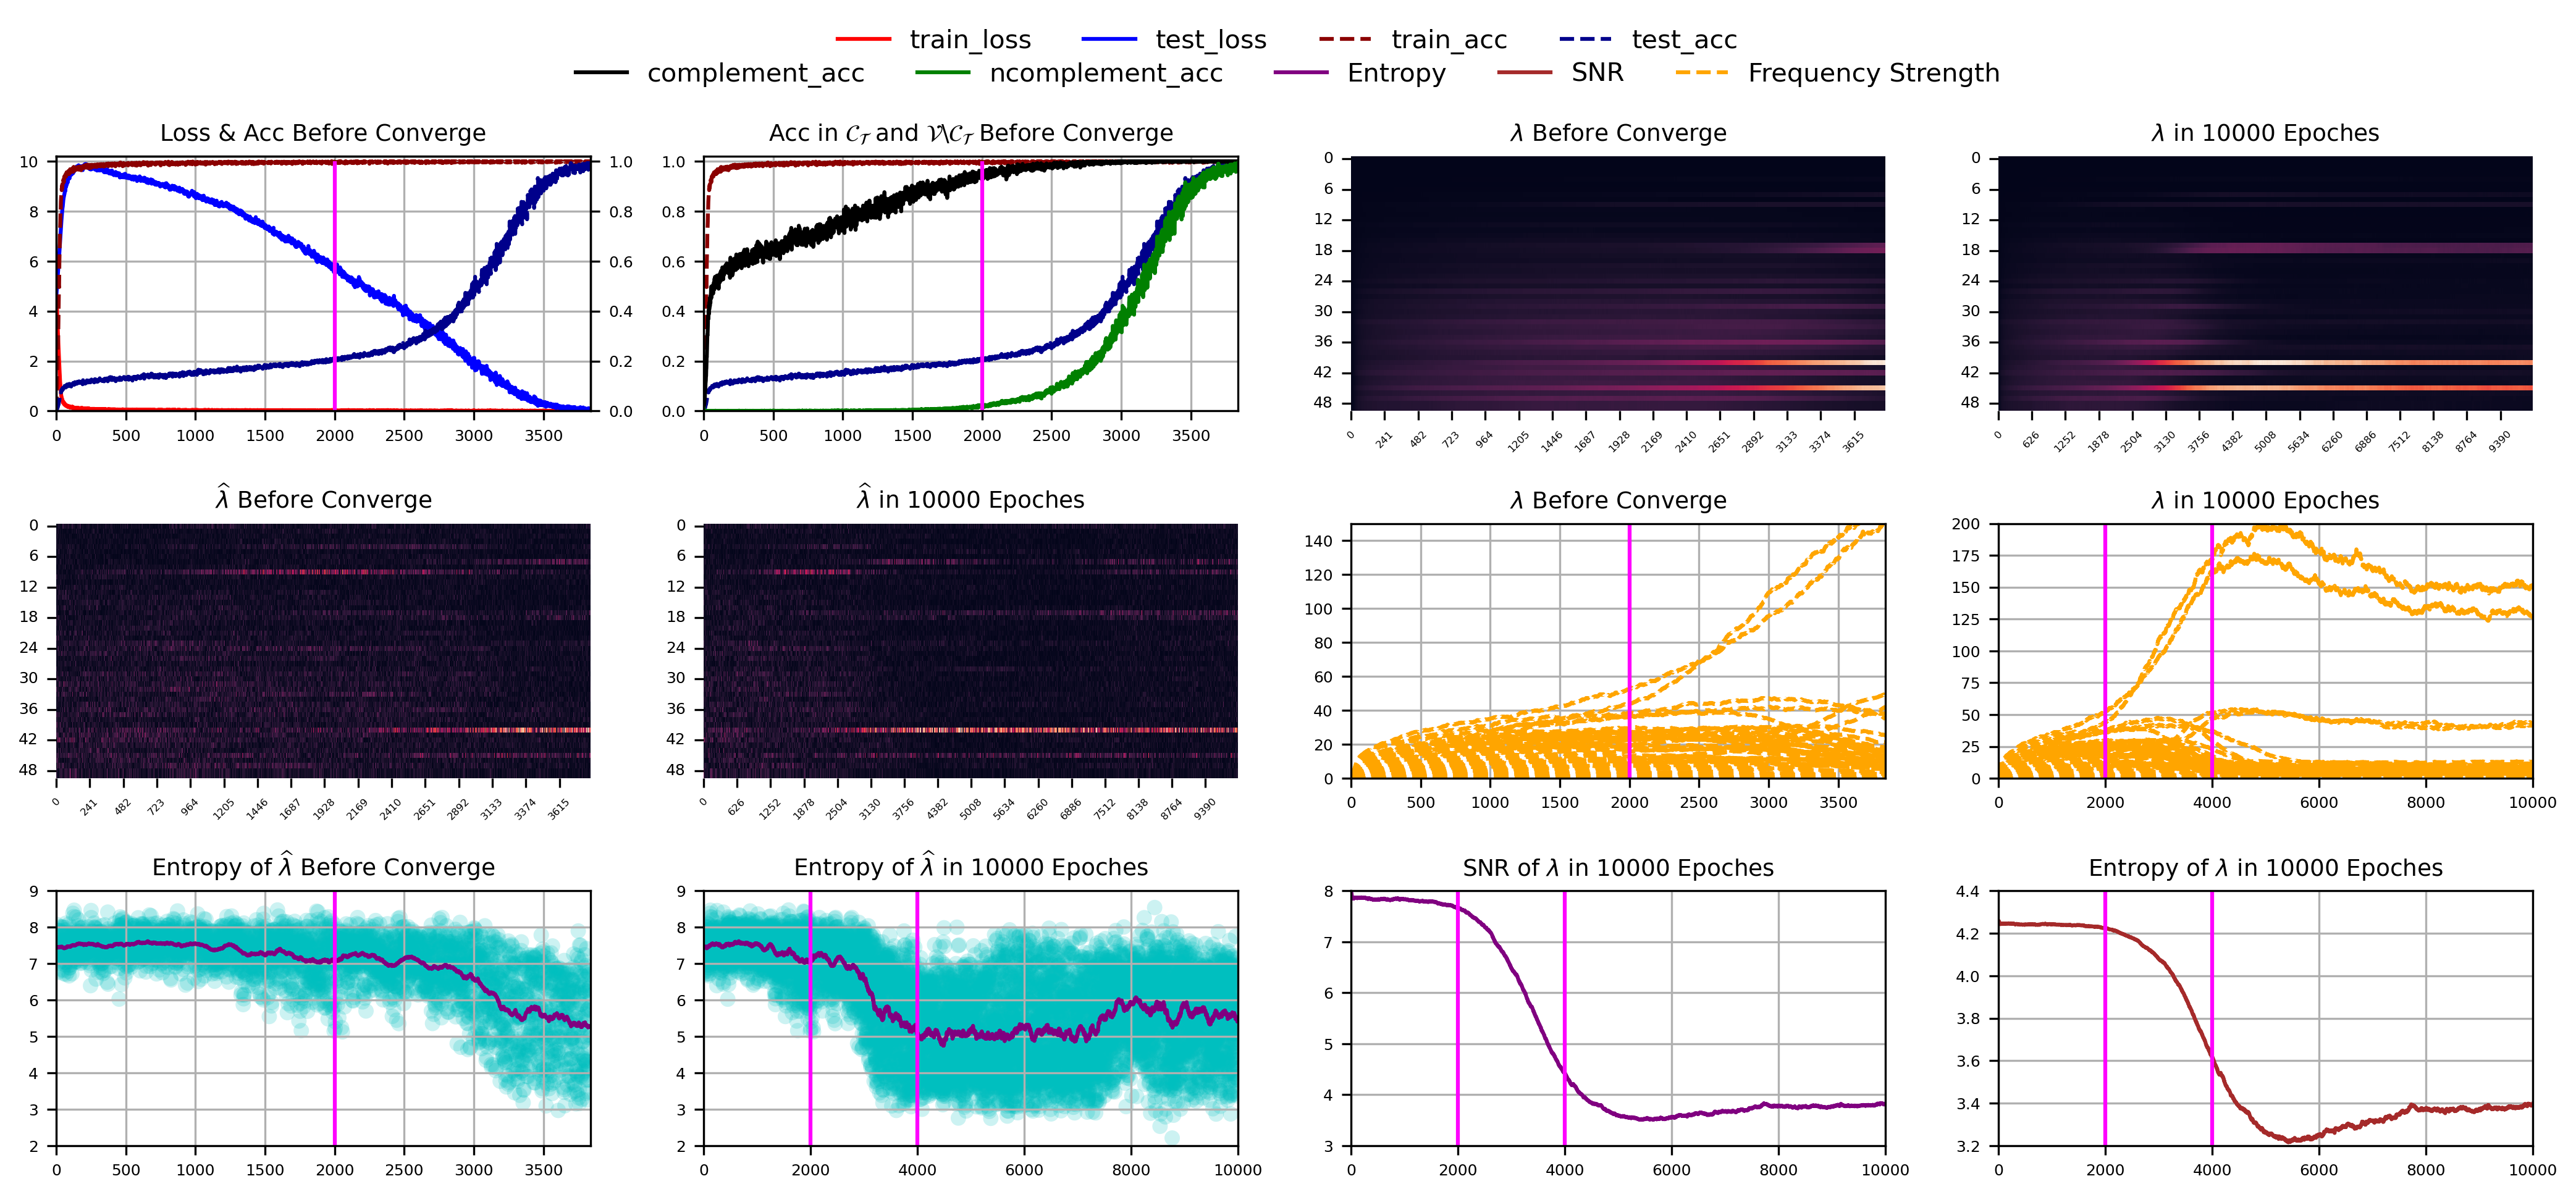
\includegraphics[width=\textwidth]{./pic/f.png}
  \caption{Outputs Both Before Convergence and Throughout the Entire Process}
  \label{f}
\end{figure}

\begin{itemize}
    \item Before about 2000 epochs, the model is learning to fit $\mathcal{T}$ and generalize to $\mathcal{C_T}$, which is consistent with \eqref{3step}. In this stage, we see that all $\lambda_i$ are of about the same level. Both the SNR and Entropy of $\bm\lambda$ and $\bm{\widehat{\lambda}}$ are almost unchanged. It seems that $\bm W$ is a mixture of all frequencies with no apparent structure.

    \item During 2000-4000 epochs, the model begins to generalize to $\mathcal{V}\backslash\mathcal{C_T}$. The heatmap indicates that approximately two frequencies begin to dominate, with all others tending towards zero. Or equivalently, $\bm\lambda$ is evolving into a "two-hot" vector. As a result, the SNR and Entropy of $\bm\lambda$ decrease rapidly in this stage. Moreover, from the heatmap of $\bm{\widehat\lambda}$ we deduce that $\bm{\widehat\lambda}$ is becoming a one-hot vector. This partly explains why the $\widehat{\bm w}_i$ is arranged circularly in $\mathbb{R}^2$.

    \item After 4000 epochs, the model converges and the accuracy on $\mathcal{V}$ oscillates around 99\%. In this stage, we can see that all but four $\lambda_i$ converge to zero. Among the four frequencies, two has been increasing since grokking, while the other two start to increase as the model approaches convergence. In the end, all frequencies tend to stabilize, resulting in the model exhibiting a regular structure.
\end{itemize}



%%%%%%%%%%%%%%%%%%%%%%%%%%%%%%%%%%%%%%%%%%%%%%%%%%%%%%%%%%%%

\newpage
\begin{small}
    \bibliography{ref}
\end{small}

\appendix


\section{Appendix}

\subsection{Notation}
\label{appendix-notation}

We first list the notations about the datasets.

\begin{itemize}
    \item $\mathcal{D}$: The dataset for modular addition on $\mathbb{Z}_p$. $\mathcal{D} = \lbrace \left( x, p, y, p+1\right)\left.\right| 0 \leqslant x, y\leqslant p-1\rbrace$. We usually treat $\mathcal{D}$ and $\mathbb{Z}_p^2$ as identical, and view $\left( x, p, y, p+1\right) \in \mathcal{D}$ the same as $(\overline{x}, \overline{y}) \in \mathbb{Z}_p^2$.

    \item $\mathcal{D}_k$: The dataset for modular $k$-addition on $\mathbb{Z}_p$. $\mathcal{D}_k = \lbrace \left(x_1, x_2,\dots, x_k, =\right) \left.\right| 0 \leqslant x_i \leqslant p-1\rbrace$.

    \item $\mathcal{T}$: The training set.

    \item $\mathcal{V}$: The testing set (validation set).

    \item $\mathcal{C_T}$: The complement of $\mathcal{T}$ in the sense of symmetry. $\mathcal{C_T} = \lbrace \left.(\overline{x}, \overline{y})\ \right|\ (\overline{x}, \overline{y}) \notin \mathcal{T}\ \text{and}\ (\overline{y}, \overline{x}) \in \mathcal{T}\rbrace$. That is, if we define the operation $S: \mathcal{D} \to \mathcal{D},\ S((\overline{x}, \overline{y})) = (\overline{y}, \overline{x})$, then $\mathcal{C_T} = S(\mathcal{T}) \backslash \mathcal{T}$. $\mathcal{C_T} = \varnothing$ is equivalent to $\mathcal{T} = S(\mathcal{T})$, which means $\mathcal{T}$ is invariant under $S$. Namely, $\mathcal{T}$ is symmetric with respect to $\overline{x}$ and $\overline{y}$.

    \item $\mathcal{A_T}$: The invariant part of $\mathcal{T}$ in the sense of symmetry. $\mathcal{A_T} = \lbrace\left.(\overline{x}, \overline{y})\ \right|\ (\overline{x}, \overline{y}) \in \mathcal{T}\ \text{and}\ (\overline{y}, \overline{x}) \in \mathcal{T}\rbrace$. This can be expressed as $\mathcal{A_T} = \mathcal{T}\cap S(\mathcal{T})$.

    \item $\mathcal{Z}_q$: The set of tuples of the form $(\overline{x}, \overline{q})$. $\mathcal{Z}_q(\mathcal{S}) = \lbrace(\overline{x},\overline{q}) \in \mathcal{S}\rbrace$. Note that $(\overline{q}, \overline{x})$ is not contained, because when testing the $\overline{q}$ addition we only check whether $\overline{x} +\overline{q} = \overline{x+q}$ instead of $\overline{q} + \overline{x} = \overline{q+x}$.
\end{itemize}

Then we list the $\gamma$s we use in Subsection \ref{abel}.
\begin{itemize}
    \item $\gamma_1 = \#\mathcal{C_T} /\#\mathcal{V}$. If the testing accuracy maintains at $\gamma_1$, it is probably that the model has generalized to $\mathcal{C_T}$ and is waiting for grokking.

    \item $\gamma_2 = \#\mathcal{Z}_0(\mathcal{T}\cup\mathcal{C_T}) / \#\mathcal{Z}_0(\mathcal{D})$. When the model generalized to $\mathcal{C_T}$, the accuracy of $\overline{0}$ addition will reach $\gamma_2$.

    \item $\gamma_3 = \#\mathcal{A_T}/\#\mathcal{D}$. If the accuracy of commutativity maintains at $\gamma_3$, it means that the model cannot learn anything except the training set $\mathcal{T}$.

    \item $\gamma_4 = \#\mathcal{Z}_0(\mathcal{T})/\#\mathcal{Z}_0(\mathcal{D})$. If the accuracy of $\overline{0}$ addition maintains at $\gamma_3$, it means that the model cannot learn anything except the training set $\mathcal{T}$.
\end{itemize}

Then we list the notations we use when discussing the frequencies.

\begin{itemize}
    \item $\bm W$: The weight of the output layer in our models.

    \item $\bm{w}_i$: The $i$th row of $\bm W$. $\bm{w}_i$ can be viewed as the representation for $\overline{i}$ in latent space.

    \item $\widehat{\bm{w}}_i$: The t-SNE projection of $\bm{w}_i$ in $\mathbb  {R}^2$.

    \item $\Delta_i$: The difference between two neighboring $\bm{w}_i$. $\Delta_i = \bm{w}_i - \bm{w}_{i-1}$. Specifically we have $\Delta_0 = \bm{w}_0 - \bm{w}_{p-1}$.

    \item $\widehat\Delta_i$: The difference between two neighboring $\widehat{\bm{w}}_i$. $\widehat\Delta_i = \widehat{\bm{w}}_i - \widehat{\bm{w}}_{i-1}$.

    \item $a_{ij}$: The inner product between two $\Delta_i$. $a_{ij} = \langle \Delta_i, \Delta_j\rangle_2$.

    \item $l_k$: The average of $a_{ij}$ along the diagonal. $l_k = \sum_{\overline{j}-\overline{i}=\overline{k}}a_{ij} /p$. If we let $A$ to be the matrix with elements $a_{ij}$, then $l_k$ is just the average of $a_{ij}$ along the $k$th diagonal of $A$.

    \item $\lambda_i$: The $i$th frequency of $\bm l$. $\lambda_s = \sum_{i=0}^{p-1} l_i\cos i\theta_s$ where $\theta_s = \frac{2s\pi}{p}$. Since $\theta_s + \theta_{p-s} = 2\pi$, we have $\lambda_{s} = \lambda_{p-s}$.
    
    \item $\widehat\lambda_i$: The $i$th frequency of $\bm\Delta$. $\widehat\lambda_s = \sum_{i=0}^{p-1} \Delta_i\cos i\theta_s$ where $\theta_s = \frac{2s\pi}{p}$. Since $\theta_s + \theta_{p-s} = 2\pi$, we have $\widehat\lambda_{s} = \widehat\lambda_{p-s}$.
\end{itemize}

\subsection{Models}
\label{appendix-model}

The structure of our models is shown in Fig \ref{modules}. All models take the general scheme on the left with different processing modules. The modules for Transformers and MLPs are displayed in detail, and for LSTM we directly use the modules implemented in Pytorch. The transformer we use has 2 layers of processing modules with 4 heads, while MLP has 3 layers and LSTM has 2 layers.

\begin{figure}[htbp]
  \centering
  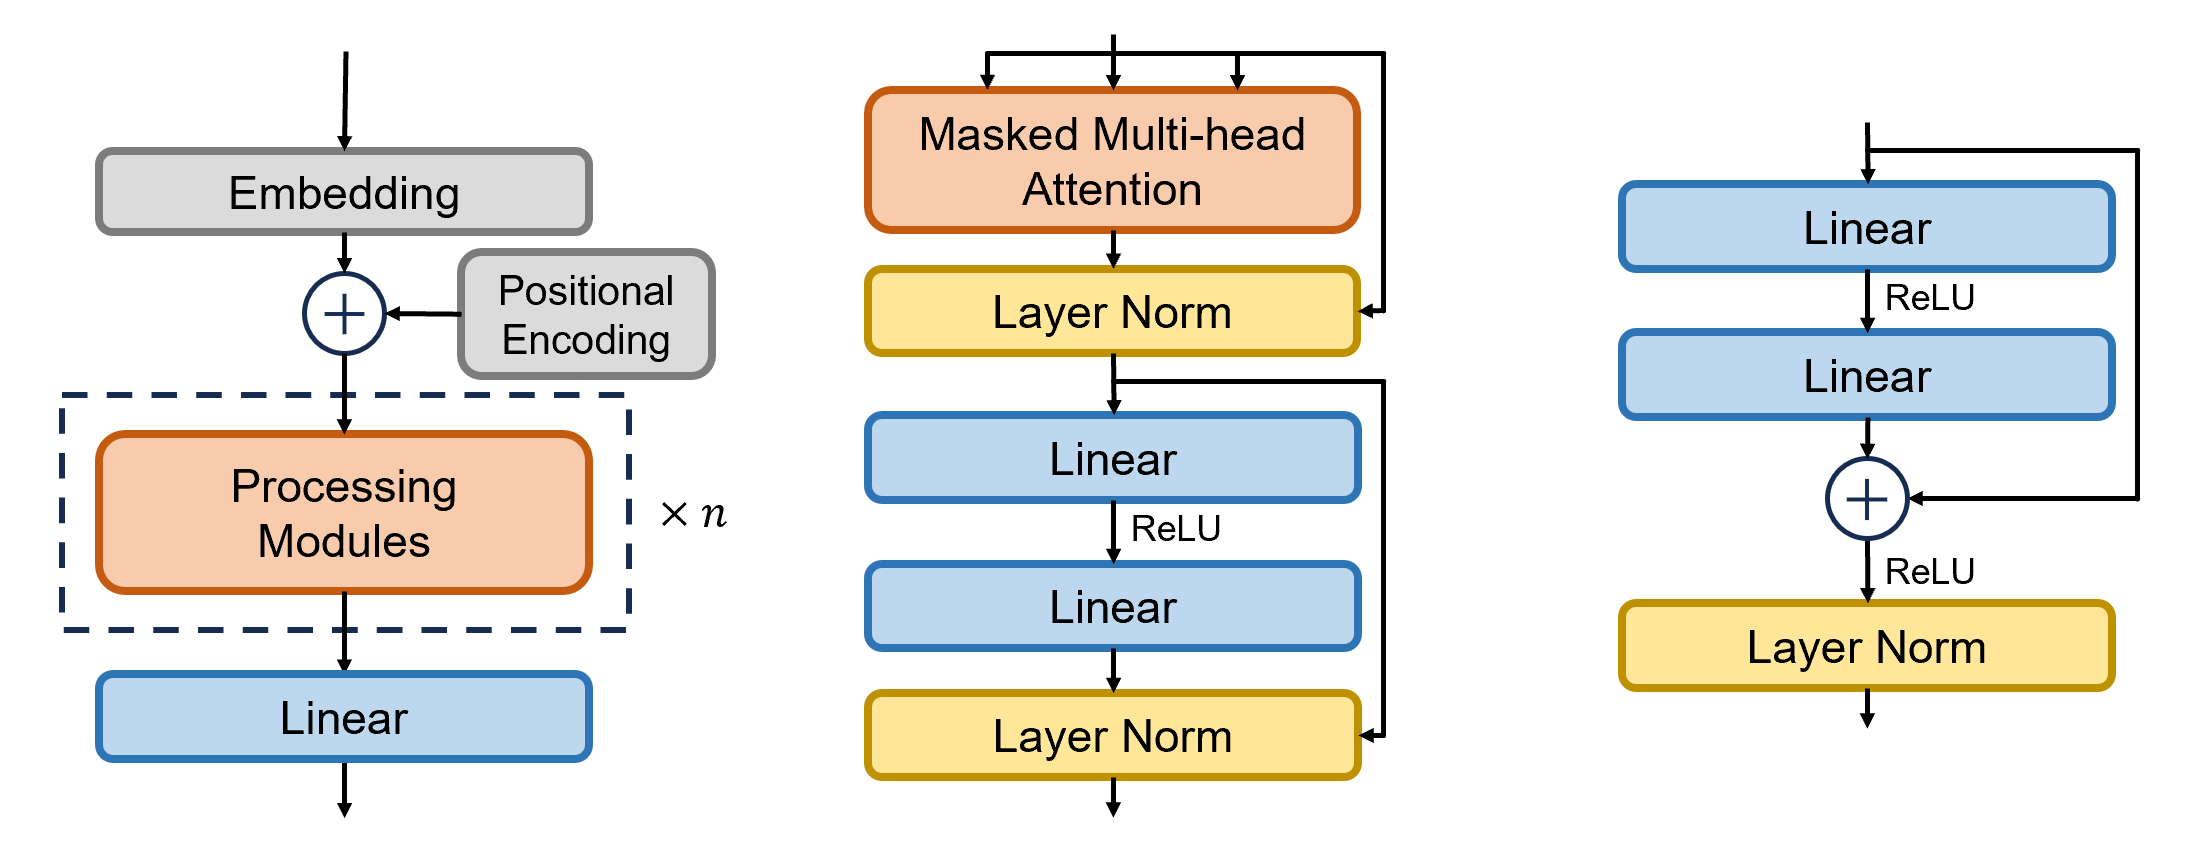
\includegraphics[width=.72\textwidth]{./pic/module.png}
  \caption{Models for Training. \textbf{Left.} General model scheme where the processing modules are to be specified. \textbf{Center.} Modules of Transformers. \textbf{Right.} Modules of MLPs.}
  \label{modules}
\end{figure}

In addition, for Transformer and LSTM, the predicted token is the last token of the output. But since MLP cannot process sequences directly, we concatenate the embedded vectors into one before sent into MLP modules. Then the predicted token of MLP is just the output.

\subsection{Replication of Figure \ref{adding}}
\label{appendix-repeat}

We use $(p = 97, \alpha = 0.2, \text{Transformer})$ with the same optimizer and parameters as in Sec \ref{models}. We execute four experiments and plot the results in Fig \ref{repeat1}. $\gamma_1$ in these four tests is $\frac{1478}{7528}, \frac{1470}{7528}, \frac{1491}{7528}, \frac{1511}{7528}$ separately, and $\gamma_2$ is $\frac{27}{97}, \frac{29}{97}, \frac{42}{97}, \frac{45}{97}$. We observe the same phenomena as in Subsec \ref{abel}. In the first step of \eqref{3step}, the model generalizes to $\mathcal{C_T}$. In this phase, the accuracy on $\mathcal{C_T}$ steadily reaches to nearly 100\%, the testing accuracy attains $\gamma_1$ and the accuracy of $\overline{0}$ addition attains $\gamma_2$. When the accuracy on $\mathcal{C_T}$ is sufficient high, the model generalizes to $\mathcal{V}\backslash\mathcal{C_T}$. All accuracies in row 2 of Fig \ref{repeat1} increase simultaneously in this stage.

\begin{figure}[htbp]
  \centering
  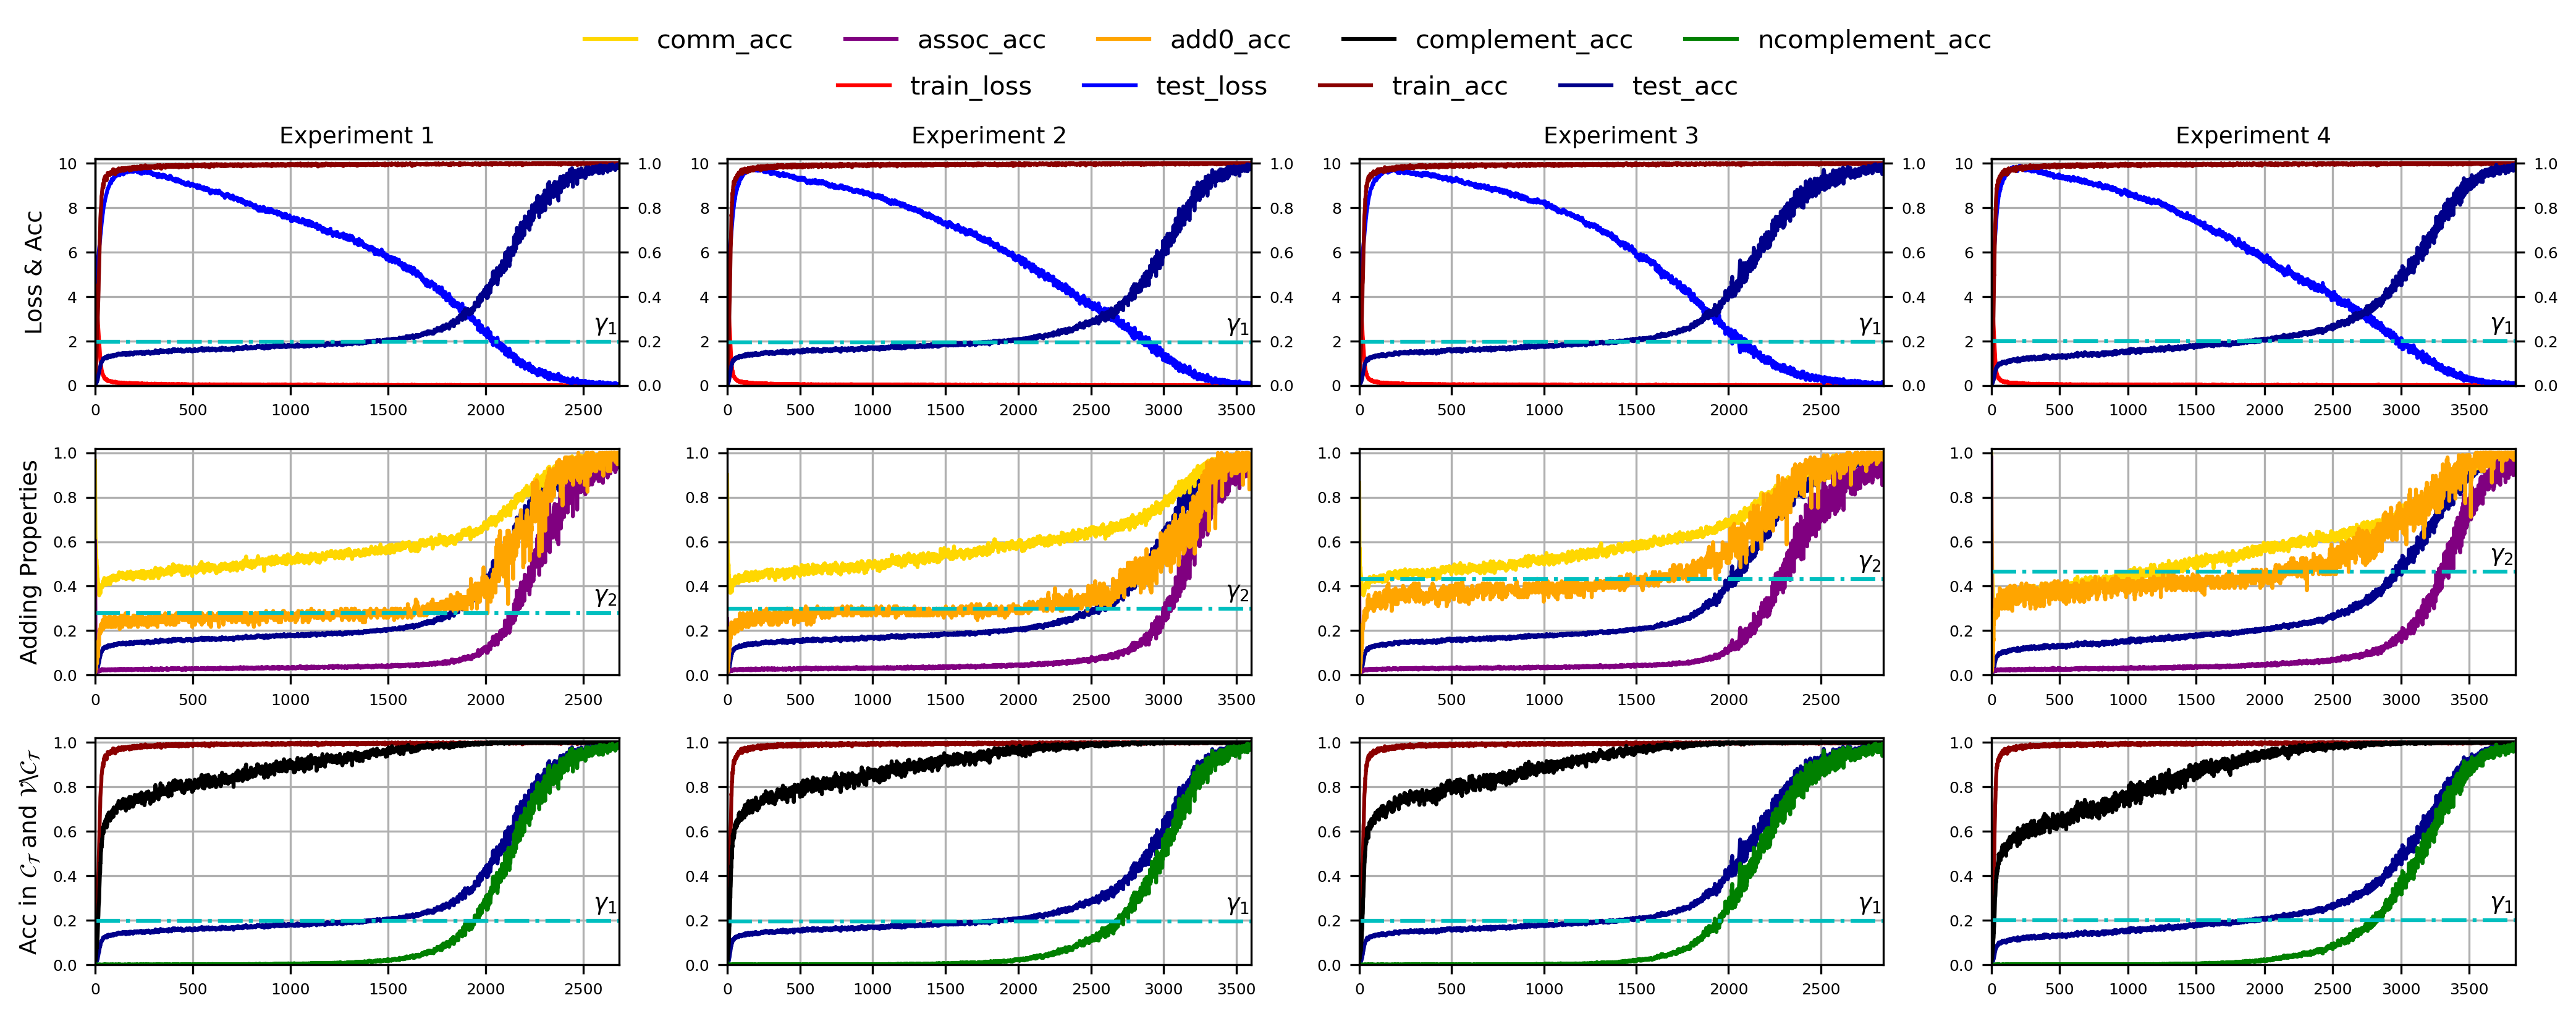
\includegraphics[width=\textwidth]{./pic/ap1.png}
  \caption{Results of Repeat Tests}
  \label{repeat1}
\end{figure}

\subsection{Learning Curves for Figure \ref{grid}}
\label{appendix-grid}

We display the learning curves corresponding to Fig \ref{grid} in Fig \ref{gridacc}. $\gamma_1$ for $\mathcal{C_T} \neq \varnothing$ and $\mathcal{C_T} = \varnothing$ is $\frac{1737}{7057}, 0$ and $\gamma_2$ is $\frac{41}{97}, \frac{23}{97}$.

\begin{figure}[htbp]
  \centering
  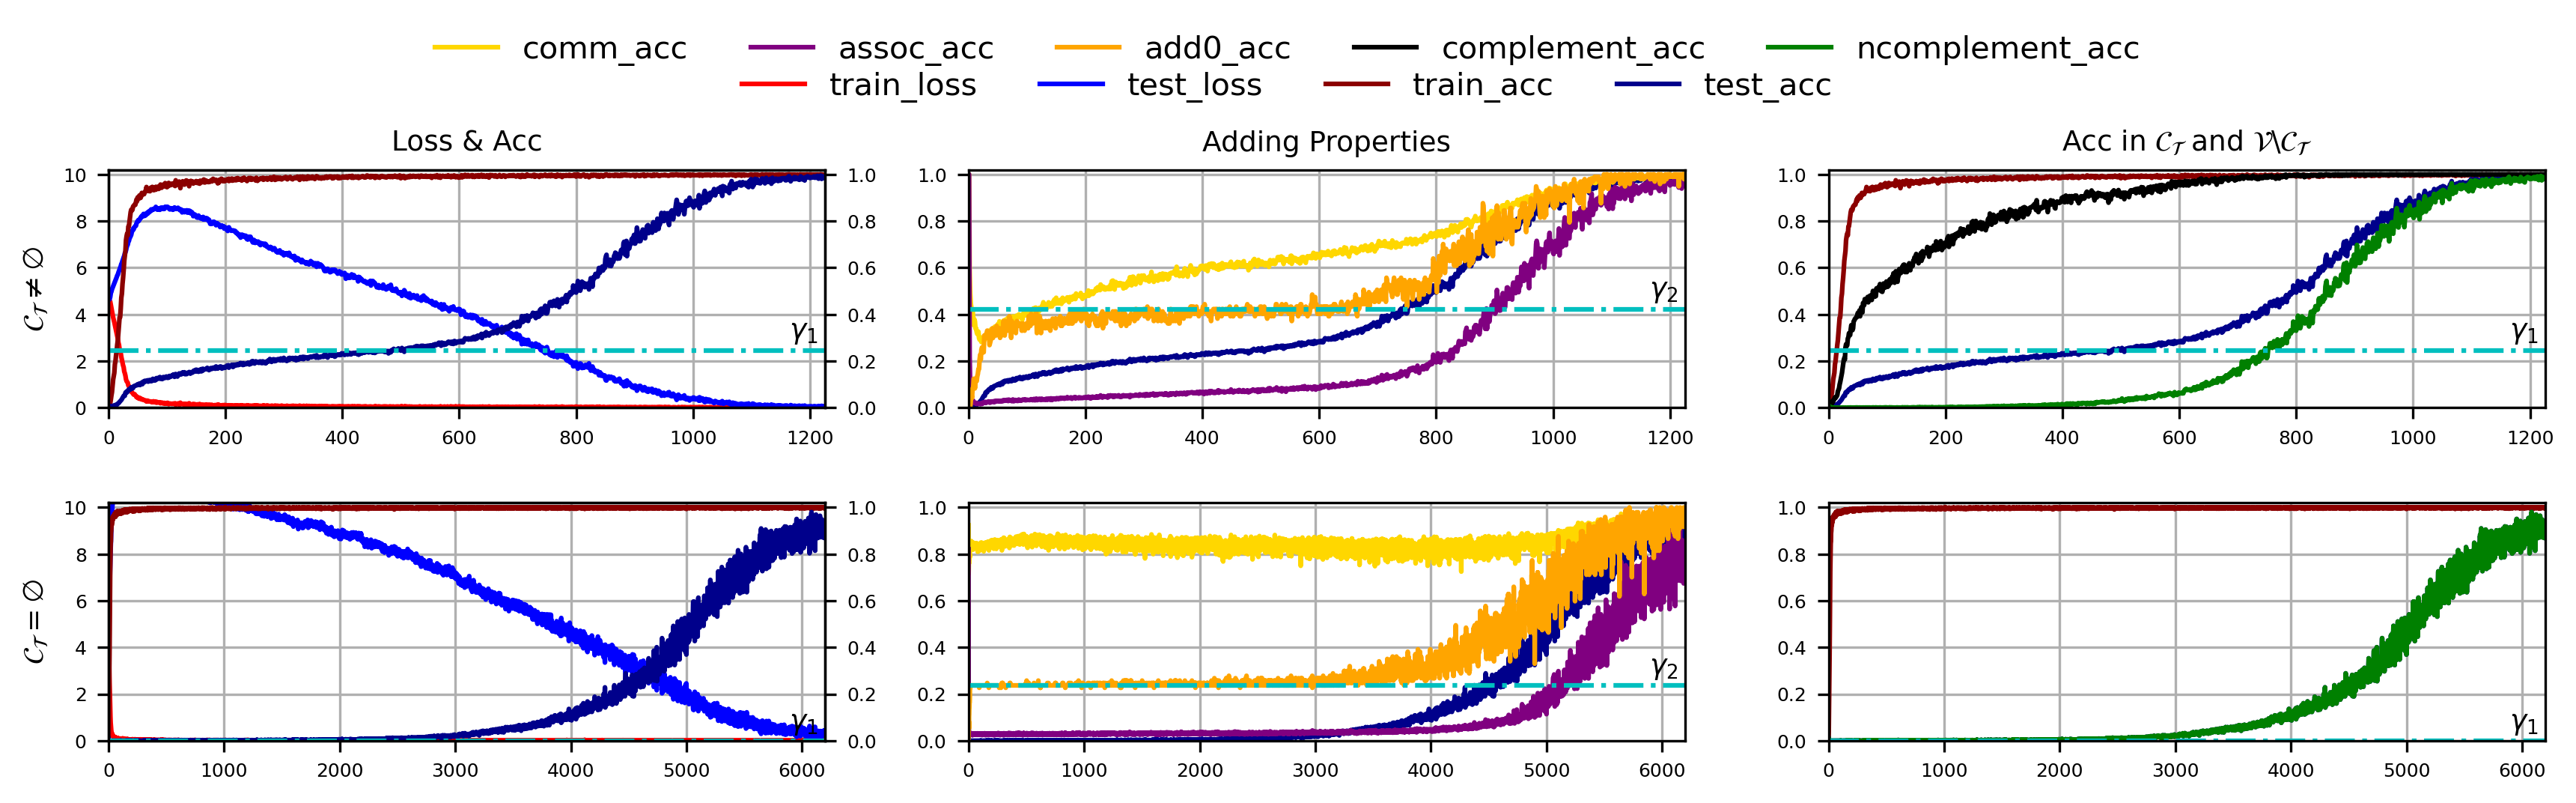
\includegraphics[width=\textwidth]{./pic/grid_acc.png}
  \caption{Learning Curves for Figure \ref{grid}}
  \label{gridacc}
\end{figure}

\subsection{Frequency}
\label{appendix-circulant}

In Fig \ref{aij}, we show the change of $A = (a_{ij})$ in an experiment. We use $(\text{Transformer}, p=97,\alpha=0.2)$ as our model. It is apparent that $A$ is becoming approximately circulant and the variance of diagonals of $A$ is getting larger as evolving.

\begin{figure}[htbp]
  \centering
  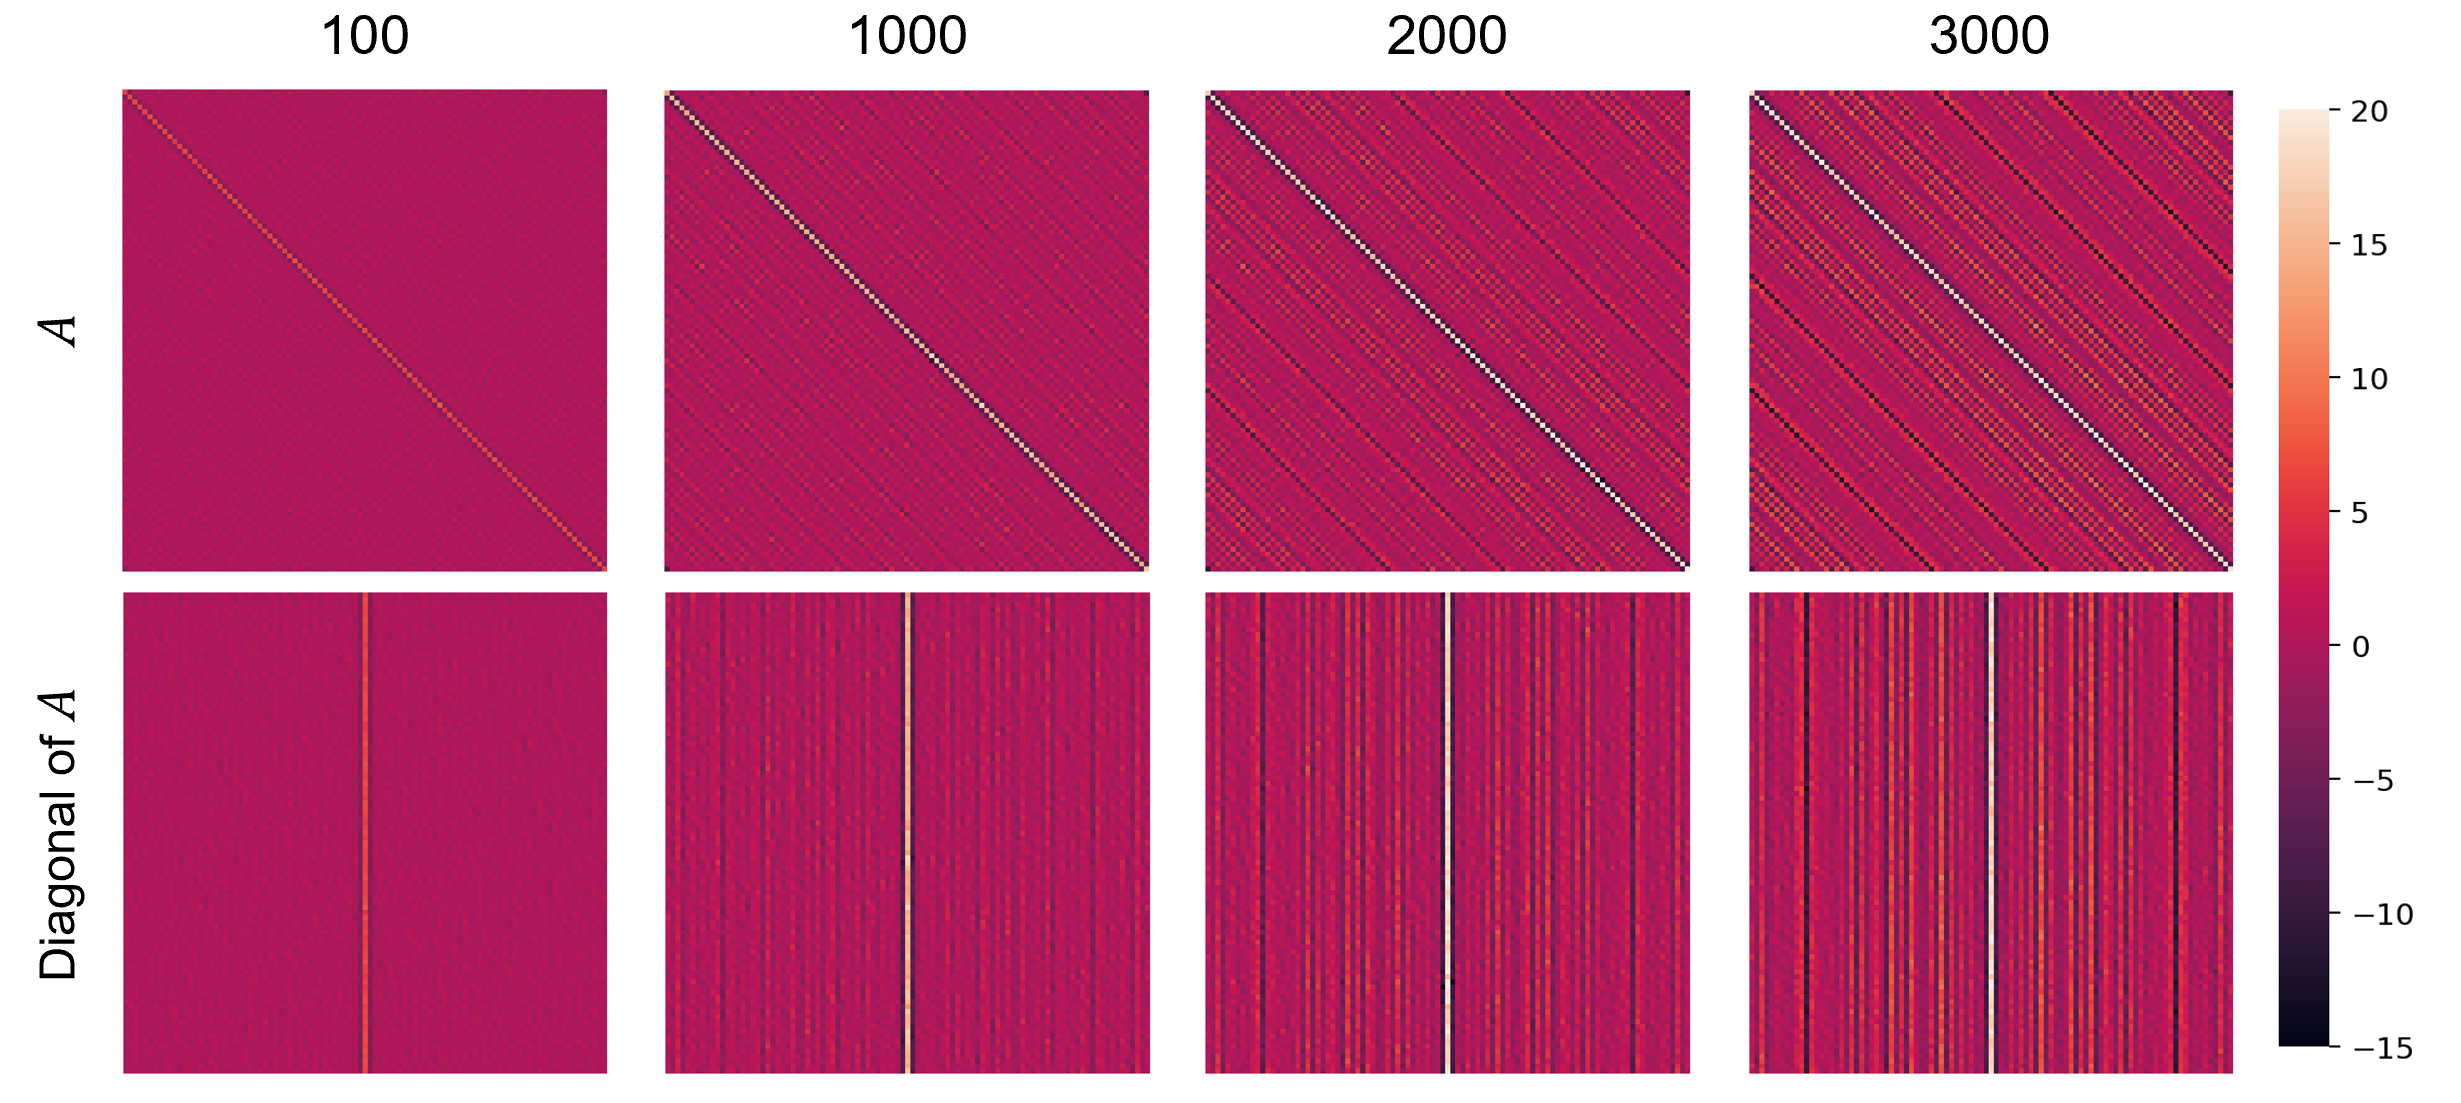
\includegraphics[width=.8\textwidth]{./pic/aij.png}
  \caption{Changes of $A$}
  \label{aij}
\end{figure}


\end{document}